%&../settings/preamble.main

\ifsubfile
\usepackage{../settings/subfile}
\setcounter{chapter}{2}

\usepackage[newfloat, cachedir=_minted-cache, outputdir=../build]{minted}
\usepackage{../libraries/set-minted}

% arara: pdflatex: { options: ["--output-directory=../build"], shell: yes, draft: yes, synctex: no }
% arara: pdflatex: { options: ["--output-directory=../build"], shell: yes, synctex: no }
\begin{document}
\fi
\chapter{Analisi delle funzioni di costo}

Abbiamo concluso la prima parte delle lezioni che ci introduceva alle equazioni di ricorrenza: ora andremo a capire i fondamenti matematici che ci permetteranno di analizzarne una famiglia più grande.

% NOTE ripasso della notazione asintotica e della complessità degli algoritmi e dei problemi.
\section{Proprietà della notazione asintotica}

\subsection{Regola generale}

\begin{theorem}[regola generale]
\(f(n) = a_k n^k + a_{k-1} n^{k-1} + \ldots a_1 n + a_0, a_k >0 \Rightarrow f(n) = \Theta(n^k)\)
\end{theorem}

\begin{proof}
\textbf{Limite superiore}: \(\exists c>0, \exists m \geqslant 0: f(n) \leqslant cn^k, \forall n \geqslant m\)

\[\begin{WithArrows}
f(n) &= a_k n^k + a_{k-1} n^{k-1} + \ldots + a_1 n + a_0 \Arrow{\(a_k > 0\) per def., rendo gli altri positivi}\\
	 &\leqslant a_k n^k + \abs{a_{k-1}} n^{k-1} +  \ldots  + \abs{a_1} n + \abs{a_0} \Arrow{\(\forall n \geqslant 1\), elevo tutte le potenze a \(k\)} \\
	 &\leqslant a_k n^k + \abs{a_{k-1}} n^k +  \ldots  + \abs{a_1} n^k + \abs{a_0} n^k \Arrow{raccolgo \(n^k\)}\\
	 &= (a_k + \abs{a_{k-1}}  +  \ldots  + \abs{a_1} + \abs{a_0})\, n^k \Arrow{esiste una costante \(c\)\\che rende la disequazione vera?} \\
	 &\stackrel{?}{\leqslant} cn^k
\end{WithArrows}\]
che è vera per \(c \geqslant (\abs{a_k} + \abs{a_{k-1}} + \ldots + \abs{a_1} + \abs{a_0} )\) (il coefficiente) e per \(m = 1\).
\end{proof}

\begin{proof}
\textbf{Limite inferiore}: \(\exists d>0, \exists m \geqslant 0: f(n) \geqslant d n^k, \forall n \geqslant m\)
\[\begin{WithArrows}
	f(n) &= a_k n^k + a_{k-1} n^{k-1} + \ldots + a_1 n + a_0 \Arrow[tikz={text width=4cm}]{normalizzo aggiungendo un segno negativo}\\
	&\geqslant a_kn^k - \abs{a_{k-1}} n^{k-1} - \ldots  - \abs{a_1} n - \abs{a_0} \Arrow{\(\forall n \geqslant 1\), elevo alla \(k-1\)}\\
	&\geqslant a_kn^k - \abs{a_{k-1}} n^{k-1} - \ldots  - \abs{a_1} n^{k-1} - \abs{a_0} n^{k-1} \\
	&\stackrel{?}{\geqslant} d n^k
\end{WithArrows}\]
L'ultima equazione è vera se:
\[
d \leqslant a_k - \frac{\abs{a_{k-1}}}{n} - \frac{\abs{a_{k-2}}}{n} -\ldots - \frac{\abs{a_1}}{n} - \frac{\abs{a_0}}{n} > 0
\iff
n > \frac{\abs{a_{k-1}} + \ldots + \abs{a_0}}{a_k} = m\qedhere
\]
% Costituito da una componente positiva (\(a_k\)) e da una componente negativa che per valori crescenti di \(n\) tende a \(0\).
\end{proof}
Abbiamo dimostrato sia il limite superiore che quello inferiore, possiamo affermare che è un \(\Theta\).

Ad esempio \(17n^3 - 47n^2 + 123n + 17 = \Theta(n^3)\).
Oppure \(2n^3 + 7 = \Theta(n^2)\).

\subsection{Funzioni di costo particolari}

La complessità di \(f(n) = 5\) è pari a \(\Theta(1)\), questa classe di complessità rappresenta quegli algoritmi che sono così ben congegnati che indipendentemente dalla dimensione dell'input impiegano un tempo costante a risolvere il problema.
Ad esempio richiedere il minimo in un vettore ordinato.

Dimostriamolo.
\begin{align*}
f(n) &= 5 \geqslant c_1 n^0 \Rightarrow c_1 \leqslant 5 \\
f(n) &= 5 \leqslant c_2 n^0 \Rightarrow c_2 \geqslant 5 \\
f(n) &= \Theta(n^0) = \Theta(1) \\
\end{align*}

La complessità di \(f(n) = 5 + \sin(n)\) è pari a \(\Theta(1)\), in quanto \(\sin(n)\) oscilla fra \(1\) e \(-1\).

\begin{figure}[H]\centering
	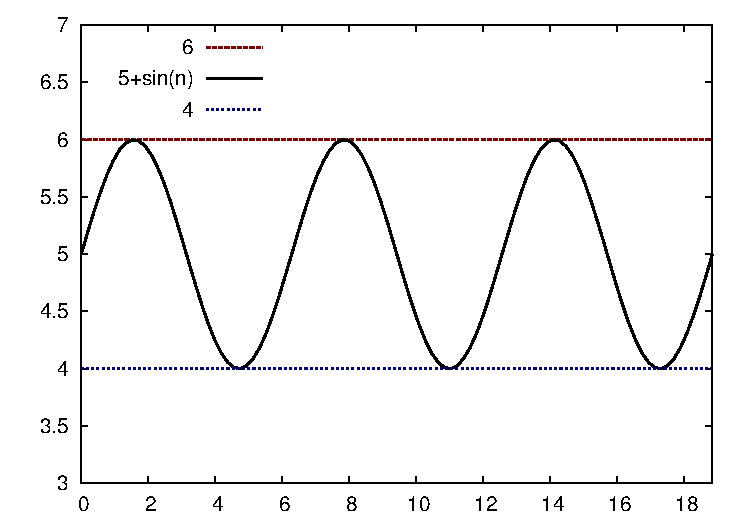
\includegraphics[width=.6\textwidth]{plot-2}
	\caption[]{\(\sin(n)\) oscilla fra \(1\) e \(-1\).}
	\label{fig:plot-2}
\end{figure}


\subsection{Proprietà delle notazioni}

\begin{theorem}[dualità]
Se \(f(n)\) è limitata superiormente da \(g(n)\), allora \(g(n)\) è limitata inferiormente da \(f(n)\).
\[ f(n) = \mathcal{O}(g(n)) \Leftrightarrow g(n) = \Omega(f(n)) \]
\end{theorem}
La dimostrazione avviene tramite passaggi algebrici.
\begin{proof}
\[\begin{WithArrows}
	f(n) = \mathcal{O}(g(n)) %
	&\Leftrightarrow f(n) \leqslant \bs{c}\ g(n), \forall n \geqslant m %
	\Arrow{ribalto la disequazione, \(c>0\)} \\
	&\Leftrightarrow g(n) > \bs{\frac{1}{c}}\: f(n), \forall n \geqslant m %
	\Arrow{rinomino \(\frac{1}{c}\) a \(c'\)} \\
	&\Leftrightarrow g(n) > \bs{c'}\, f(n), \forall n \geqslant m, c' = \frac{1}{c} %
	\Arrow{passo alla notazione dei quantificatori} \\
	&\Leftrightarrow g(n) = \Omega(f(n))
\end{WithArrows}\]
\end{proof}

\begin{theorem}[eliminazione delle costanti]
\[\begin{WithArrows}
f(n) = \Omicron(g(n)) \Leftrightarrow af(n) = \Omicron(g(n)), \forall a > 0 \\
f(n) = \Omega(g(n)) \Leftrightarrow af(n) = \Omega(g(n)), \forall a > 0
\end{WithArrows}\]
\end{theorem}
La dimostrazione avviene sempre tramite semplici passaggi algebrici.
\begin{proof}
\[\begin{WithArrows}
f(n) = \Omicron(g(n)) &\Leftrightarrow f(n) \leqslant c\,g(n), \forall n \geqslant m \Arrow{Introduco una costante \(a\)}\\
	  &\Leftrightarrow f(n) \leqslant ac\,g(n), \forall n \geqslant m, \forall a \geqslant 0 \Arrow{raccolgo \(ac\) sotto un'unica costante \(c'\)}\\
	  &\Leftrightarrow f(n) \leqslant c'g(n), \forall n \geqslant m, c' = ac > 0 \Arrow{per definizione}\\
	  &\Leftrightarrow a f(n) = \Omicron(g(n))
\end{WithArrows}\]
\end{proof}

Ad esempio \(2 \log n = \Theta(\log n)\), ignoriamo quindi le costanti numeriche.

\begin{theorem}[sommatoria, sequenza di algoritmi]
	\begin{align*}
	&
	\begin{dcases}
	f_1(n) = \Omicron(g_1(n)) \\
	f_2(n) = \Omicron(g_2(n)) \\
	\end{dcases}
	\Rightarrow f_1(n) + f_2(n) = \Omicron(\maxFunction(g_1(n),g_2(n)))\\
	&
	\begin{dcases}
	f_1(n) = \Omega(g_1(n)) \\
	f_2(n) = \Omega(g_2(n)) \\
	\end{dcases}
	\Rightarrow f_1(n) + f_2(n) = \Omega(\maxFunction(g_1(n),g_2(n)))\\
	\end{align*}
\end{theorem}
\begin{proof}
\[\begin{WithArrows}
f_1 (n) = \Omicron(g_1 (n)) \land f_2 n = \Omicron(g_2(n)) &\Rightarrow \Arrow{per definizione}\\
f_1 (n) \leqslant c_1 g_1 (n) \land f_2 (n) \leqslant c_2 g_2 (n) &\Rightarrow \Arrow[jump=2]{raccolgo}\\
f_1 (n) + f_2 (n) \leqslant c_1 g_1 (n) + c_2 g_2 (n) &\Rightarrow\\
f_1 (n) + f_2 (n) \leqslant \maxFunction\{c_1, c_2\}(2 \cdot \maxFunction(g_1(n), g_2(n)) &\Rightarrow \Arrow{per definizione}\\
f_1 (n) + f_2 (n) = \Omicron(g_1(n) + g_2(n))
\end{WithArrows}\]
\end{proof}

Ad esempio se ripeto due volte un algoritmo lineare, l'algoritmo risultante sarà comunque lineare.
Mentre se ho un algoritmo lineare ed un algoritmo quadratico, la complessità risultante è una combinazione delle due, il limite superiore della complessità totale sarà quindi quadratica.

\begin{theorem}[cicli annidati]
Se \(f_1(n)\) viene ripetuto \(f_2(n)\) volte, allora \(f_1(n) \cdot f_2(n)\) è limitato superiormente dal prodotto delle complessità e limitato inferiormente dal prodotto delle complessità.
\begin{align*}
	&
	\begin{dcases}
	f_1(n) = \Omicron(g_1(n)) \\
	f_2(n) = \Omicron(g_2(n)) \\
	\end{dcases}
	\Rightarrow f_1(n) \cdot f_2(n) = \Omicron(g_1(n) \cdot g_2(n))\\
	&
	\begin{dcases}
	f_1(n) = \Omega(g_1(n)) \\
	f_2(n) = \Omega(g_2(n)) \\
	\end{dcases}
	\Rightarrow f_1(n) \cdot f_2(n) = \Omega(g_1(n) \cdot g_2(n))\\
\end{align*}
\end{theorem}
La dimostrazione è molto semplice.
\begin{proof}
\[\begin{WithArrows}
f_1 (n) = \Omicron(g_1 (n)) \land f_2 n = \Omicron(g_2(n)) &\Rightarrow \Arrow{per definizione}\\
f_1 (n) \leqslant c_1 g_1 (n) \land f_2 (n) \leqslant c_2 g_2 (n) &\Rightarrow \Arrow{raccolgo, \(c_1 c_2 > 0\)}\\
f_1 (n) \cdot f_2 (n) \leqslant c_1 c_2 g_1(n) g_2(n)
\end{WithArrows}\]
\end{proof}

Ad esempio, se ripeto \(n\) volte un algoritmo di costo \(\log n\), l'algoritmo complessivo avrà un costo di \(n \log n\).

\begin{theorem}[simmetria]
Se \(f(n)\) è limitata superiormente ed inferiormente da \(g(n)\), allora anche \(g(n)\) è limitata inferiormente e superiormente da \(f(n)\).
	\[ f(n) = \Theta(g(n)) \Leftrightarrow g(n) = \Theta(f(n)) \]
\end{theorem}

Vuol dire semplicemente che \(2n^2 + 7 = \Theta(n^2) \Leftrightarrow n^2 = \Theta(2n^2 + 7)\).

La dimostrazione avviene tramite la proprietà di dualità:
\begin{proof}
\[\begin{WithArrows}
f(n) = \Theta(g(n)) &\quad\Rightarrow\quad f(n) = \Omicron(g(n)) \quad\Rightarrow\quad g(n) = \Omega(f(n)) \\
f(n) = \Theta(g(n)) &\quad\Rightarrow\quad f(n) = \Omega(g(n)) \quad\Rightarrow\quad g(n) = \Omicron(f(n))
\end{WithArrows}\]
\end{proof}

\begin{theorem}[transitività]
Se \(f(n)\) è limitata superiormente da \(g(n)\), e \(g(n)\) è limitata superiormente da \(h(n)\), allora \(f(n)\) è limitata superiormente da \(h(n)\).
\[
\begin{dcases}
f(n) = \mathcal{O}(g(n)) \\
g(n) = \mathcal{O}(h(n)) \\
\end{dcases}
\Rightarrow f(n) = \Omicron(h(n))
\]
\end{theorem}
La dimostrazione è banale:
\begin{proof}
\[\begin{WithArrows}
	f(n) = \mathcal{O}(g(n)) \land g(n) = \mathcal{O}(h(n)) &\Rightarrow %
	\Arrow{applico la definizione} \\
	f(n) \leqslant c_1 g(n) \land g(n) \leqslant c_2 h(n) &\Rightarrow %
	\Arrow{sostituisco \(g(n)\) con \(c_2 h(n)\)} \\
	f(n) \leqslant c_1 c_2 h(n) &\Rightarrow %
	\Arrow{\(c_1 c_2 > 0\), elimino la costante} \\
	f(n) = \mathcal{O}(h(n))
\end{WithArrows}\]
\end{proof}

\subsection*{Altre funzioni di costo}

Vogliamo provare che \fbox{\(\log n = \Omicron(n)\)}

Dimostriamo per induzione che \(\exists c > 0, \exists m \geqslant 0\,\colon \log n \leqslant cn, \forall n \geqslant m\).

\begin{itemize}
	\item \textbf{caso base} \((n=1)\):
	\[\begin{WithArrows}
	\log n &\leqslant cn \Arrow{\(n = 1\)}\\
	\log 1 &\leqslant c \cdot 1 \Arrow{semplifico}\\
	0 &\leqslant c
	\end{WithArrows}\]
	\item \textbf{ipotesi induttiva}: \(\log k \leqslant ck, \forall k \leqslant n\)
	\item \textbf{passo induttivo} dimostriamo la proprietà per \(n+1\):
	\[\begin{WithArrows}
	\log(n+1) \leqslant \log(n+n) &= \log2n \quad \forall n \geqslant 1 \Arrow{\(\log ab = \log a + \log b\)}\\
	&= \log 2 + \log n \Arrow{\(\log_2 2 = 1\)}\\
	&= 1 + \log n \Arrow{per ipotesi induttiva}\\
	&\leqslant 1 + cn \Arrow{obiettivo}\\
	&\overset{?}{\leqslant} c(n+1) \Arrow{metto a confronto}\\
	1 + cn &\leqslant c(n+1) \Arrow{moltiplico}\\
	1 + \Ccancel{cn} &\leqslant \Ccancel{cn} + c \Arrow{semplifico}\\
	1 &\leqslant c
	\end{WithArrows}\]
\end{itemize}

\subsection*{Classificazione delle funzioni}

\`{E} possibile trarre un ordinamento dalle principali espressioni, estendendo le relazioni che abbiamo dimostrato fino ad ora.
Per ogni \(r < s, h < k, a < b\):
\[
\Omicron(1)
\subset
\Omicron(\log^r n)
\subset
\Omicron(\log^s n)
\subset
\Omicron(n^h)
\subset
\Omicron(n^h \log^r n)
\subset
\Omicron(n^h \log^s n)
\subset
\Omicron(n^k)
\subset
\Omicron(a^n)
\subset
\Omicron(b^n)
\]

Ricordati che \(\log^r(n) = {(\log n)}^r\).
Non è detto che gli esponenti siano interi.
\(\sqrt[1000]{n}\) cresce più velocemente di \(\log^2 n\).
\(n\) cresce meno velocemente di \(n \log n\), il quale a sua volta cresce meno velocemente di \(n \log^2 n\).

\clearpage
\section{Analisi per livelli}

Nell'analisi per livelli (o dell'albero di ricorsione) andiamo sostanzialmente a \enquote{srotolare} la ricorrenza in un albero, i cui nodi rappresentano i costi dei vari livelli della ricorsione.

\subsection{Esempi di analisi per livelli}

\subsubsection*{Analisi per livelli dell'algoritmo della ricerca binaria}

Equazione di ricorrenza della ricerca binaria:
\[
	T(n) =
	\begin{dcases}
		T(\nicefrac{n}{2}) + b & n > 1 \\
		1 & n \leq 1 \\
	\end{dcases}
\]

Assumiamo per semplicità che \(n = 2^k\), ovvero che \(k = \log n\).
\`{E} possibile quindi risolvere questa ricorrenza nel seguente modo:
\[\begin{WithArrows}
T(n) &= b + T(\frac{n}{2}) \Arrow{\(T\left(\frac{n}{2} \cdot \frac{1}{2} \right) + b\)}\\
	 &= b + b + T(\frac{n}{4}) \Arrow{\(T\left(\frac{n}{4} \cdot \frac{1}{2} \right) + b\)}\\
	 &= b + b + b + T(\frac{n}{8}) \Arrow[jump=2]{svolgo \(\log n\) operazioni}\\
	 &\phantom{= b + b + b}\vdots\\
	 &= \underbracket[0.01mm]{b + b + \ldots + b }_{\log n}+ T(1) \Arrow{semplifico}\\
	 &= b\log n + T(1) \Arrow{eliminazione delle costanti}\\
	 &= \Theta(\log n)
\end{WithArrows}\]

\subsubsection*{Analisi per livelli del primo tentativo della moltiplicazione di Karatsuba}

Equazione di ricorrenza:
\[
	T(n) =
	\begin{dcases}
		4 T(n/2) + n & n > 1 \\
		1 & n \leqslant 1 \\
	\end{dcases}
\]

\`{E} possibile risolvere questa ricorrenza nel modo seguente:
\[\begin{WithArrows}[displaystyle]
T(n) &= n + 4T(\nicefrac{n}{2}) \Arrow{\(4T\left(\frac{n}{2} \cdot \frac{1}{2} \right) + \frac{n}{2}\)}\\
	 &{\color{gray}= n + 4\left(4T\left(\frac{n}{2} \cdot \frac{1}{2}\right) + \frac{n}{2} \right)} \Arrow[tikz={color=gray}]{semplifico}\\
	 &= n + 4\nicefrac{n}{2} + 16 T(\nicefrac{n}{4}) \Arrow{\(4T\left(\frac{n}{4} \cdot \frac{1}{2} \right) + \frac{n}{4}\), \(4\nicefrac{n}{2} = 2n\)}\\
	 &{\color{gray} n + 2n + 16\left(4T\left(\frac{n}{4} \cdot \frac{1}{2}\right) + \frac{n}{4} \right)} \Arrow[tikz={color=gray}]{semplifico}\\
	 &= n + 2n + 16\nicefrac{n}{4} + 64 T(\nicefrac{n}{8}) \Arrow[jump=2]{svolgo \(\log n\) operazioni}\\
	 &\phantom{= n + 2n + 16}\vdots \\
	 &= \underbracket[0.01mm]{n + 2n + 4n + 8 n + \cdots + 2^{\log n-1}n}_{sommatoria} + 4^{\log n} T(1) \Arrow{raccolgo}\\
	 &= n \sum_{j=0}^{\log n-1} 2^j + 4^{\log n}
\end{WithArrows}\]

Ciò che abbiamo ottenuto è una forma chiusa, non più un'equazione di ricorrenza: non è ancora nella sua forma definitiva, dobbiamo ancora trattarla.

\[\begin{WithArrows}[displaystyle]
T(n) &= n \sum_{j=0}^{\log n-1} 2^j + 4^{\log n} \Arrow{Applico \(\forall x \neq 1: \sum_{j=0}^k x^j = \frac{x^{k+1}-1}{x-1}\),\\ dove \(k = \log n-1\)}\\[2ex]
	 &= n \cdot \frac{2^{\log n}-1}{2-1} + 4^{\log n} \Arrow{\(2^{\log n} = n^{\log_2 2} = n^{1}\)}\\
	 &= n(n-1) + 4^{\log n} \Arrow{moltiplico: \(n(n-1) = n^2 - n\)\\semplifico: \(4^{\log n} = n^{\log 4} = n^2\)}\\[2ex]
	 &= n^2 - n + n^2 \Arrow{raccolgo \(n^2\)}\\
	 &= 2n^2 - n \Arrow{regola generale}\\
	 &= \Theta(n^2)
\end{WithArrows}\]

Possiamo concludere che \(T(n) = n + 4T(\nicefrac{n}{2}) = \Theta(n^2)\).

\clearpage
\subsection*{Modifichiamo l'esempio precendente}

Esaminiamo la seguente equazione di ricorrenza:
\[
T(n) =
\begin{dcases}
	4T(\nicefrac{n}{2}) + n^3 & n > 1 \\
	1 & n \leqslant 1
\end{dcases}
\]

Per semplicità consideriamo \(n = 2^{\ell}\).
\begin{center}
\begin{tabular}{@{} *{5}{c} @{}}
	\toprule
		livello & dim. & costo chiam. & no. chiamate & costo livello \\
	\midrule
		\(0\) & \(n\)   & \(n^3\)     & \(1\)  & \(n^3\) \\
	\addlinespace
		\(1\) & \(\nicefrac{n}{2}\) & \((\nicefrac{n}{2})^3\) & \(4\)  & \(4(\nicefrac{n}{2})^3\)\\
	\addlinespace
		\(2\) & \(\nicefrac{n}{4}\) & \((\nicefrac{n}{4})^3\) & \(16\) & \(16(\nicefrac{n}{4})^3\)\\
	\addlinespace
		\(3\) & \(\nicefrac{n}{8}\) & \((\nicefrac{n}{8})^3\) & \(64\) & \(64(\nicefrac{n}{8})^3\)\\
	\addlinespace
		\(\vdots\) & \(\vdots\) & \(\vdots\) & \(\vdots\) & \(\vdots\) \\
	\addlinespace
		\(i\) & \(\nicefrac{n}{2^i}\) & \((\nicefrac{n}{2^i})^3\) & \(4^i\) & \(4^i (\nicefrac{n}{2^i})^3\) \\
	\addlinespace
		\(\vdots\) & \(\vdots\) & \(\vdots\) & \(\vdots\) & \(\vdots\) \\
	\addlinespace
		\({\ell-1}\) & \(\nicefrac{n}{2^{\ell-1}}\) & \((\nicefrac{n}{2^{\ell-1}})^3\) & \(4^{\ell-1}\) & \(4^{\ell-1} (\nicefrac{n}{2^{\ell-1}})^3\) \\
	\addlinespace
		\(\ell = \log n\) & 1 & \(T(1)\) & \(4^{\log n}\) & \(4^{\log n}\) \\
	\bottomrule
\end{tabular}
\end{center}

Sommando il costo di tutti i \(\ell-1\) livelli ed il livello \(\ell\)-esimo otteniamo:
\[\begin{WithArrows}[displaystyle]
T(n) &= \sum_{i=0}^{\log n-1} 4^i \cdot \frac{n^3}{2^{3i}} + 4^{\log n} \Arrow{semplifico: \(4^i = 2^{2i}\),\\porto fuori: \(n^3\)}\\
	 &= n^3 \sum_{i=0}^{\log n-1} \frac{2^{2i}}{2^{3i}} + 4^{\log n} \Arrow{semplifico: \(\frac{2^{2i}}{2^{3i}} = {\left(\frac{1}{2}\right)}^{i}\)}\\
	 &= n^3 \sum_{i=0}^{\log n-1} {\left(\frac{1}{2}\right)}^{i} + 4^{\log n} \Arrow{cambio di base, \(4^{\log n} = n^{\log 4} = n^2\)}\\
	 &= n^3 \sum_{i=0}^{\log n-1} {\left(\frac{1}{2}\right)}^{i} + n^2 \Arrow{estensione della sommatoria ad \(\infty\)}\\
	 &\leqslant n^3 \sum_{i=0}^{\infty} {\left(\frac{1}{2}\right)}^{i} + n^2 \Arrow{Serie geometrica infinita decrescente:\\\(\forall x, \abs{x} < 1: \sum_{i=0}^{\infty} x^i = \frac{1}{1-x}\), dove \(x = \frac{1}{2}\)}\\
	 &= n^3 + \frac{1}{1-\frac{1}{2}} + n^2 \Arrow{semplifico: \(\frac{1}{1-\frac{1}{2}} = 2\)}\\
	 &= 2n^3 + n^2
\end{WithArrows}\]
Abbiamo dimostrato che \(T(n) \leqslant 2n^3 + n^2\), possiamo quindi affermare che \(T(n) = \Omicron(n^3)\), ma non possiamo affermare che \(T(n) = \Theta(n^3)\) poiché abbiamo dimostrato solo un limite superiore.

\begin{hint}
Tutte le volte che notiamo in un'equazione di riccorrenza una parte polinomiale, come ad esempio \(n^3\), possiamo dire con certezza che l'equazione è \(\Omega(n^3)\).
\end{hint}

Ora possiamo affermare che \(T(n) = \Theta(n^3)\).

\clearpage
\subsection*{Modifichiamo l'esempio precendente ulteriormente}

Esaminiamo la seguente equazione di ricorrenza:
\[
T(n) =
\begin{dcases}
	4T(\nicefrac{n}{2}) + n^2 & n > 1 \\
	1 & n \leqslant 1
\end{dcases}
\]
Cambia il costo della chiamata, che passa dall'essere \(n^3\) all'essere \(n^2\).
Di conseguenza cambia anche il costo del livello.
\begin{center}
\begin{tabular}{@{} *{5}{c} @{}}
	\toprule
		Livello & Dim. & Costo chiam. & no. chiamate & Costo livello \\
	\midrule
		\(0\) & \(n\)   & \(n^2\)     & \(1\)  & \(n^2\) \\
	\addlinespace
		\(1\) & \(\nicefrac{n}{2}\) & \((\nicefrac{n}{2})^2\) & \(4\)  & \(4(\nicefrac{n}{2})^2\)\\
	\addlinespace
		\(2\) & \(\nicefrac{n}{4}\) & \((\nicefrac{n}{4})^2\) & \(16\) & \(16(\nicefrac{n}{4})^2\)\\
	\addlinespace
		\(3\) & \(\nicefrac{n}{8}\) & \((\nicefrac{n}{8})^2\) & \(64\) & \(64(\nicefrac{n}{8})^2\)\\
	\addlinespace
		\(\vdots\) & \(\vdots\) & \(\vdots\) & \(\vdots\) & \(\vdots\) \\
	\addlinespace
		\(i\) & \(\nicefrac{n}{2^i}\) & \((\nicefrac{n}{2^i})^2\) & \(4^i\) & \(4^i (\nicefrac{n}{2^i})^2\) \\
	\addlinespace
		\(\vdots\) & \(\vdots\) & \(\vdots\) & \(\vdots\) & \(\vdots\) \\
	\addlinespace
		\({\ell-1}\) & \(\nicefrac{n}{2^{\ell-1}}\) & \((\nicefrac{n}{2^{\ell-1}})^2\) & \(4^{\ell-1}\) & \(4^{\ell-1} (\nicefrac{n}{2^{\ell-1}})^2\) \\
	\addlinespace
		\(\ell = \log n\) & 1 & \(T(1)\) & \(4^{\log n}\) & \(4^{\log n}\) \\
	\bottomrule
\end{tabular}
\end{center}

Sommando il costo di tutti i \(\ell-1\) livelli ed il livello \(\ell\)-esimo otteniamo:
\[\begin{WithArrows}[displaystyle]
T(n) &= \sum_{i=0}^{\log n-1} \frac{n^2}{2^{2i}} \cdot 4i + 4^{\log_2 n} \Arrow{semplifico: \(4^i = 2^{2i}\), \(4^{\log n} = n^{\log_2 4} = n^2\)\\porto fuori: \(n^2\)}\\
	 &= n^2 \sum_{i=0}^{\log n-1} \frac{2^{2i}}{2^{2i}} + n^2 \Arrow{semplifico: \(\frac{2^{2i}}{2^{2i}} = 1\)}\\
	 &= n^2 \sum_{i=0}^{\log n-1} 1 + n^2 \Arrow{svolgo la sommatoria: \(\sum_{i=0}^{\log n-1} 1 = \log n\)}\\
	 &= n^2 \log n + n^2 \Arrow{regola generale}\\
	 &= \Theta(n^2 log n)
\end{WithArrows}\]

\section*{Conclusioni}

Per riassumere, se consideriamo i termini non ricorrenti, \(n\) ha prodotto \(n^2\), \(n^2\) ha prodotto \(n^2 \log n\) ed \(n^3\) ha prodotto \(n^3\).
Quando avremo a disposizione lo strumento \enquote{master theorem} riusciremo semplicemente guardando l'equazione di ricorrenza a capire quale complessità essa produce.

\clearpage
\section{Metodo di sostituzione}

Vediamo ora un ulteriore meccanismo per risolvere le equazioni di ricorrenza in quanto il metodo precendente in alcuni casi può non esserci di aiuto.
Il metodo di sostituzione è un metodo in cui si cerca di \enquote{indovinare} (\foreign{guess}) una soluzione in base alla propria esperienza ed in seguito si dimostra che questa intuizione è corretta tramite dimostrazione per induzione.

\subsection*{Primo esercizio}

\[
	T(n) =
	\begin{dcases}
		T( \lfloor \nicefrac{n}{2} \rfloor ) + n & n > 1 \\
		1 & n \leqslant 1
	\end{dcases}
\]
Risolvendolo tramite il metodo precendente otteniamo:
\[\begin{WithArrows}[displaystyle]
T(n) &= n \sum_{i=0}^{\log n} {\left( \frac{1}{2} \right)}^{i} \Arrow{estensione della sommatoria ad \(\infty\)}\\
	 &\leqslant n \sum_{i=0}^{\infty} {\left( \frac{1}{2} \right)}^{i}
	 \Arrow{Serie geometrica decrescente infinita:\\
	 \(\forall x, \abs{x} < 1: \sum_{i=0}^{\infty} x^i = \frac{1}{1-x}\), dove \(x = \frac{1}{2}\)}\\
	 &\leqslant n \frac{1}{1-\frac{1}{2}} \Arrow{\(\frac{1}{1-\frac{1}{2}} = 2\)}\\
	 &= 2n
\end{WithArrows}\]

Sapendo già il risultato proviamo -- per tentativi -- a dimostrare che \fbox{\(T(n) = \Omicron(n)\)}

\textbf{Limite superiore}: Dobbiamo dimostrare che \(\exists c > 0, \exists m \geqslant 0 \,\colon T(n) \leqslant cn, \forall n \geqslant m\)
\begin{itemize}
	\item \textbf{caso base} dimostriamo \(T(1)\):
	\[T(1) = 1 \overset{?}{\leqslant} c \cdot 1 \iff c \geqslant 1\]
	\item \textbf{ipotesi induttiva} \(\forall k < n \,\colon T(n) \leqslant ck\), ossia assumiamo che per tutti i valori più piccoli di \(n\) la dimostrazione sia già stata fatta.
	\item \textbf{passo induttivo} dimostriamo la disequazione per \(T(n)\):
	\[\begin{WithArrows}
	T(n) &= T(\floor{\frac{n}{2}}) + n \Arrow{sost. ip. ind. con \(k = \floor{\frac{n}{2}}\)}\\
	&\leqslant c \floor{\frac{n}{2}} + n \Arrow{semplifico l'intero inferiore}\\
	&\leqslant c \frac{n}{2} + n \Arrow{raccolgo \(n\)}\\
	&= (\frac{c}{2} + 1)n \Arrow{obiettivo}\\
	&= (\frac{c}{2} + 1)n \overset{?}{\leqslant} cn \Arrow[jump=2]{semplifico}\\
	&\Rightarrow \frac{c}{2} + 1 \leqslant c\\
	&\Rightarrow c \geqslant 2
	\end{WithArrows}\]
	Abbiamo quindi provato che \(T(n) \leqslant cn\), con due diversi valori della nostra costante \(c\): nel caso base è risultata \(c \geqslant 1\), mentre nel passo induttivo è risultata pari a \(c \geqslant 2\).
	% Possiamo accettare solo un valore di \(c\) che \emph{rispetti entrambe le disequazioni}, in questo caso è \(c = 2\).
	Quindi la nostra ipotesi è valida per qualsiasi valore di c t.c.\ \(c \geqslant a\) e \(c \geqslant 2\), ovvero \(\forall c \geqslant 2\).

	Quanto abbiamo dimostrato vale per \(n = 1\) e per tutti i valori di \(n\) successivi, di conseguenza \(m = 1\).
\end{itemize}

Al solo scopo didattico (in quanto lo potremmo dedurlo dal termine non ricorsivo) proviamo passo passo anche il limite inferiore, ossia che \fbox{\(T(n) = \Omega(n)\)}

\textbf{Limite inferiore}: Dobbiamo dimostrare che \(\exists d > 0, \exists m \geqslant 0 \,\colon T(n) \geqslant dn, \forall n \geqslant m\).

\begin{note}
Usiamo la costante \(d\) al solo scopo di non confonderla la costante \(c\) usata nella dimostrazione precendente.
\end{note}
\begin{itemize}
	\item \textbf{caso base} \(T(1)\):
	\[T(1) = 1 \overset{?}{\geqslant} d \cdot 1 \iff d \leqslant 1\]
	\item \textbf{ipotesi induttiva} \(\forall k < n \,\colon T(k) \geqslant ck\), ossia assumiamo che per tutti i valori più piccoli di \(n\) la mia dimostrazione sia già stata fatta.
	\item \textbf{ipotesi induttiva} dimostriamo la disequazione per \(T(n)\)
	\[\begin{WithArrows}
	T(n) &= T(\floor{\frac{n}{2}}) + n \Arrow{sost. ip. ind. con \(d = \frac{n}{2}\)}\\
		 &\geqslant d \floor{\frac{n}{2}} + n \Arrow{semplifico l'intero inferiore}\\
		 &\geqslant d \frac{n}{2} - 1 + n \Arrow{raccolgo \(n\)}\\
		 &= \left( \frac{d}{2} - \frac{1}{n} + 1 \right) n \Arrow{obiettivo}\\
		 &= \left( \frac{d}{2} - \frac{1}{n} + 1 \right) n \overset{?}{\geqslant} dn \Arrow[jump=2]{semplifico}\\
		 &\Rightarrow \frac{d}{2} - \frac{1}{n} + 1 \geqslant d\\
		 &\Rightarrow d \leqslant 2 - \frac{2}{n}
	\end{WithArrows}\]

	Abbiamo quindi provato che \(T(n) \geqslant dn\), con due diversi valori della nostra costante \(d\): nel caso base è risultata \(d \leqslant 1\), mentre nel passo induttivo è risultata pari a \(d \leqslant 2 - \frac{2}{n}\).
	% Possiamo accettare solo un valore di \(d\) che \emph{rispetti entrambe le disequazioni} per ogni valore di \(n \geqslant 1\), in questo caso è \(d = 1\).
	\(d = 1\) è valore che soddisfa entrambre le disequazioni, dimostra quindi la nostra tesi.

	Quanto abbiamo dimostrato vale per \(n = 1\) e per tutti i valori di \(n\) successivi, di conseguenza \(m = 1\).

	Per concludere abbiamo provato che \(T(n) = T(\floor{\frac{n}{2}}) + n\) è limitata sia superiormente \(T(n) = \Omicron(n)\), sia inferiormente \(T(n) = \Omega(n)\), possiamo affermare quindi con assoluta certezza che \(T(n) = \Theta(n)\).
\end{itemize}

\
Nota che avremmo potuto evitare la dimostrazione del limite inferiore osservando che
\[\textstyle T(n) = T(\floor{\frac{n}{2}}) + n \geqslant n \overset{?}{\geqslant} dn\]
l'ultima disequazione risulta vera per \(d \leqslant 1\), la quale è una condizione identica a quella del caso base.
Nota che non abbiamo fatto nemmeno ricorso all'ipotesi induttiva.

\subsection*{Cosa succede se si sbaglia l'intuizione}

\[
T(n) =
	\begin{dcases}
	T(n-1) + n & n > 1\\
	1 & n \leqslant 1\\
	\end{dcases}
\]

\begin{note}
L'equazione di riccorrenza rappresenta il caso in cui selection sort sia espresso in forma ricorsiva.
\end{note}
\begin{figure}[H]
	\centering
	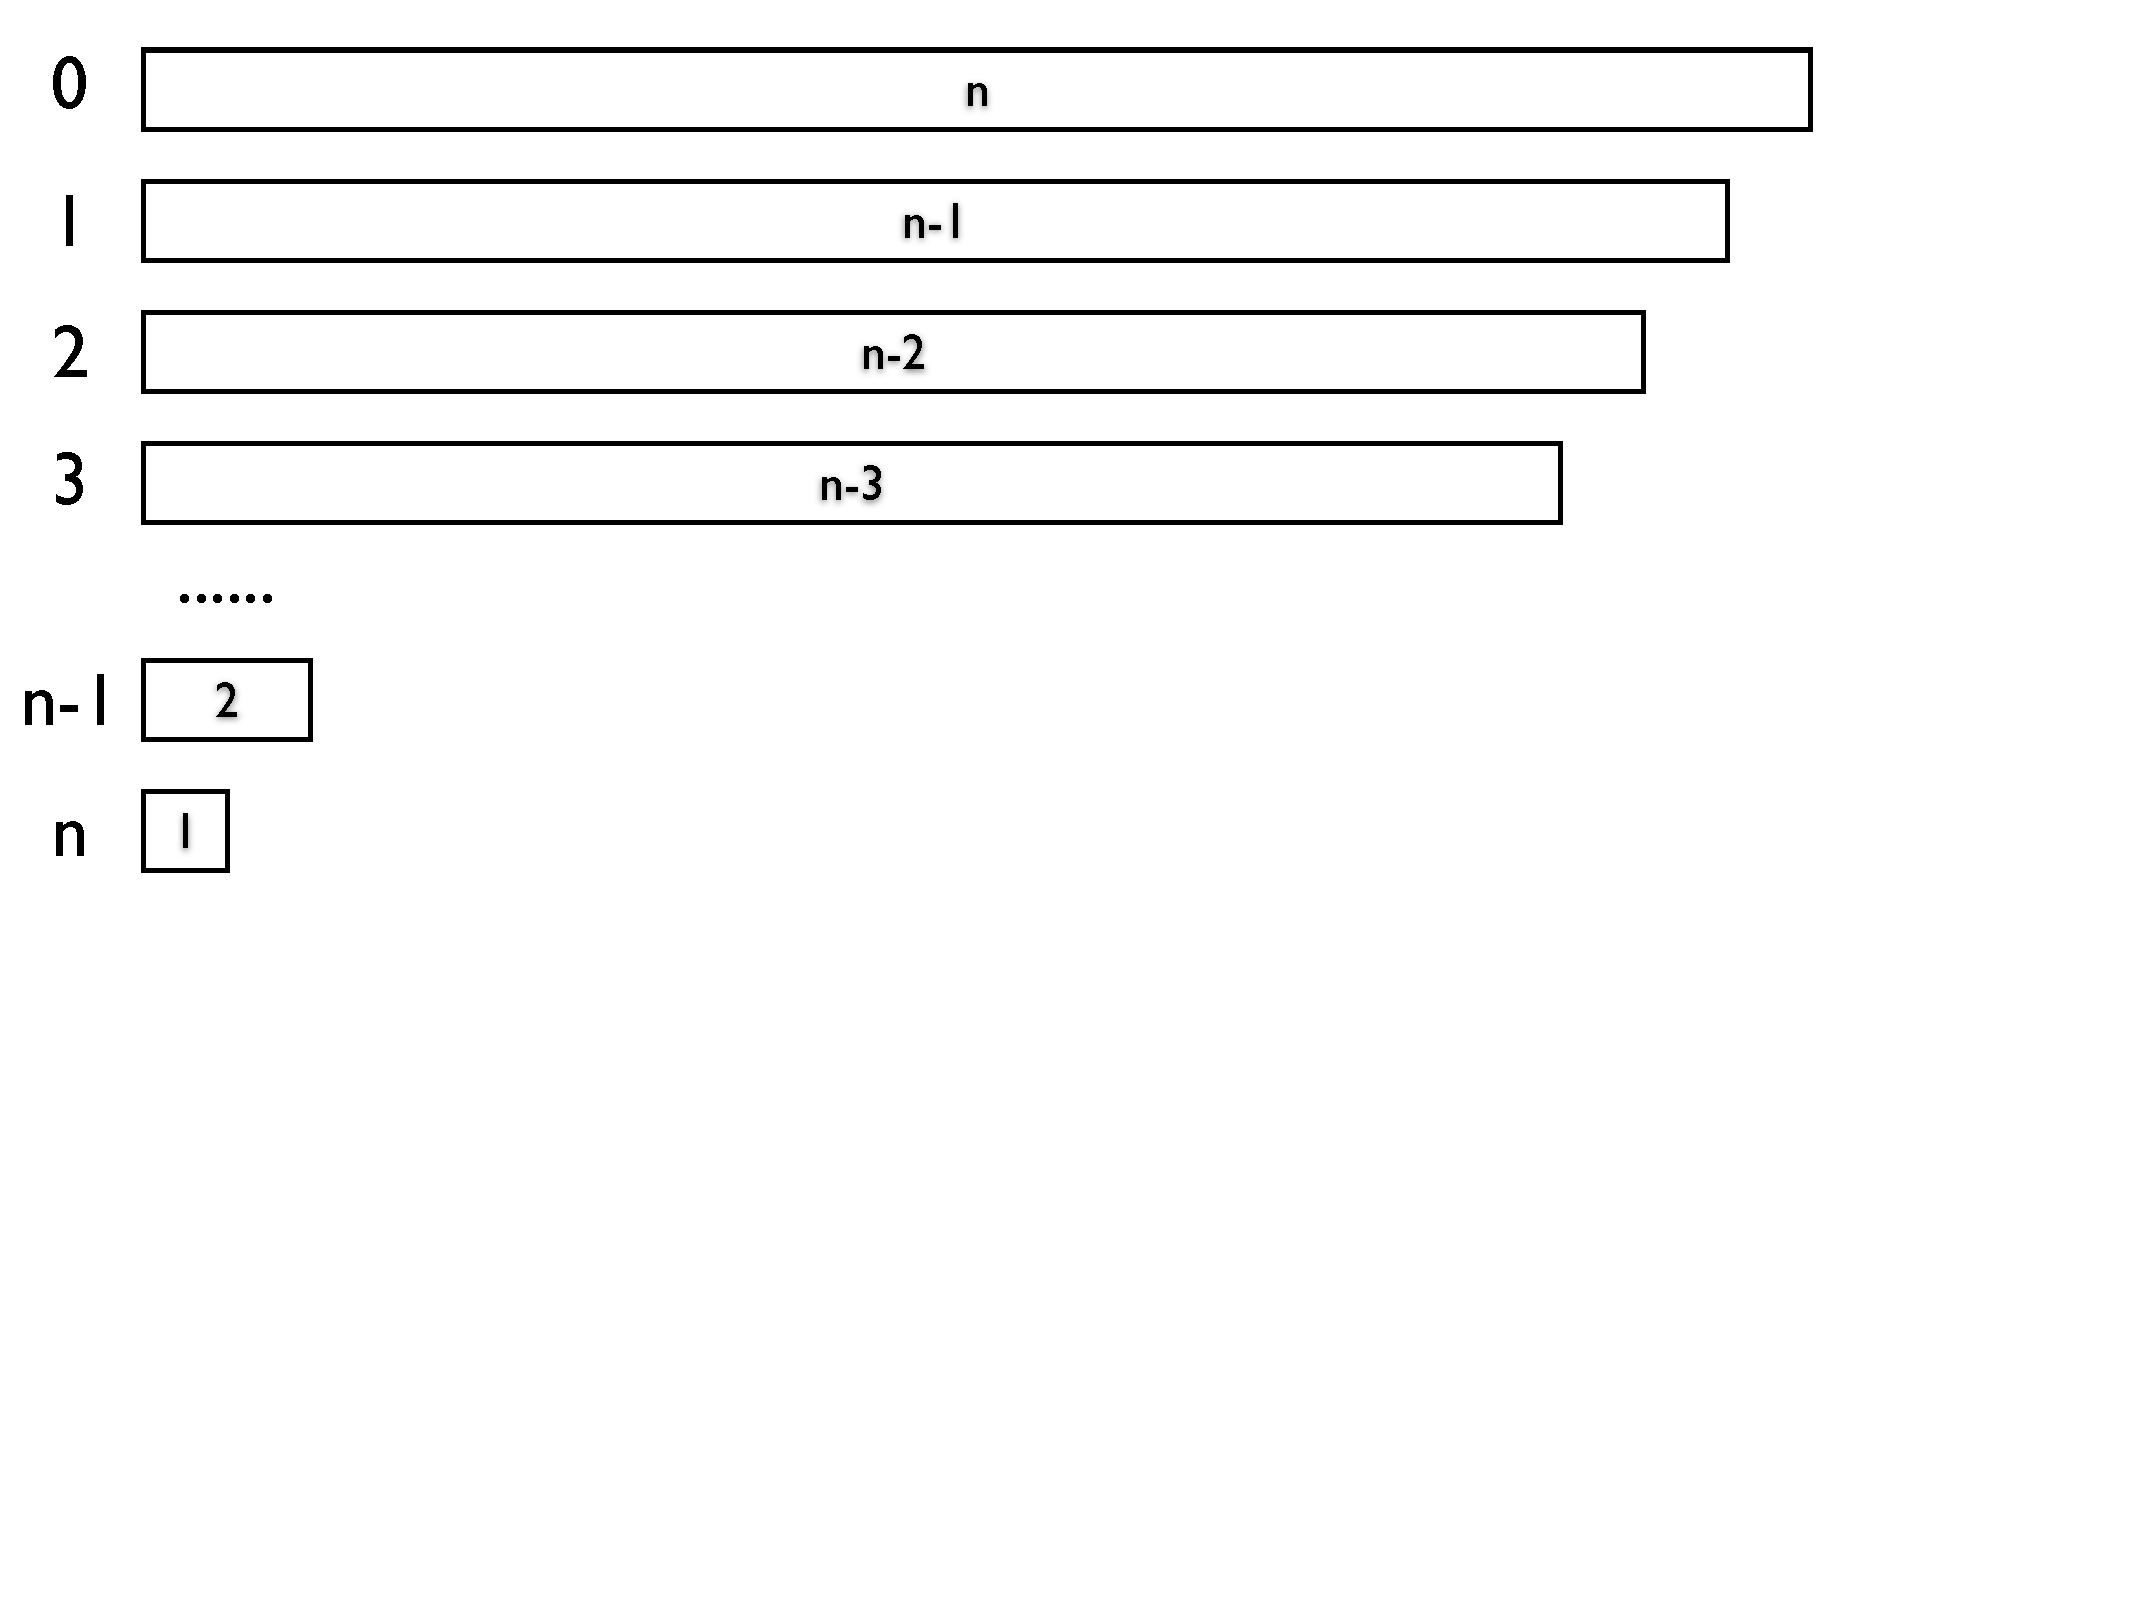
\includegraphics[width=.6\textwidth]{ennemenouno}
	\caption[]{Rappresentazione della ricorrenza lineare.}
\end{figure}

Possiamo rappresentare la funzione nel seguente modo:
\[
	T(n) = \sum_{i=1}^{n} i = \frac{n (n + 1)}{2} = \Theta(n^2)
\]

Effettuiamo un tentativo e proviamo a dimostrare che \fbox{\(T(n) = \Omicron(n)\)}

\textbf{Limite superiore}: Dobbiamo dimostrare che \(\exists c > 0, \exists m \geqslant 0 \,\colon T(n) \leqslant cn, \forall n \geqslant m\).
\begin{itemize}
	\item \textbf{caso base} lo saltiamo perché vedremmo subito che è sbagliato.
	\item \textbf{ipotesi induttiva} \(\forall k < n \,\colon T(k) \leqslant ck\).
	\item \textbf{passo induttivo} dimostriamo la disequazione per \(T(n)\):
	\[\begin{WithArrows}
	T(n) &= T(n-1) + n \Arrow{sost. ip. ind. con \(k = n-1\)}\\
	&= c(n-1) + n \Arrow{moltiplico}\\
	&= cn - c + n \Arrow{raccolgo \(n\)}\\
	&= (c+1)n - c \Arrow{rimuovo l'elemento negativo}\\
	&\leqslant (c+1)n \Arrow{obiettivo}\\
	&= (c+1)n \overset{?}{\leqslant} cn \Arrow{semplifico}\\
	&\Rightarrow c+1 \leqslant c
	\end{WithArrows}\]

	Possiamo notare che l'ultima disequazione risulta impossibile.
	Dunque quando proviamo a dimostrare qualcosa di sbagliato non riusciremo a dimostrarlo.
\end{itemize}

\subsection*{Difficoltà matematica}

\[
T(n) =
	\begin{cases}
	T(\floor{ \frac{n}{2} }) + T(\ceil{ \frac{n}{2} }) + 1 & n > 1 \\
	1 & n \leqslant 1
	\end{cases}
\]

\begin{note}
\`{E} possibile ottenere questa equazione di riccorrenza dall'algoritmo che calcola il minimo di un vettore non ordinato in maniera ricorsiva.
\end{note}

\begin{figure}[H]
	\centering
	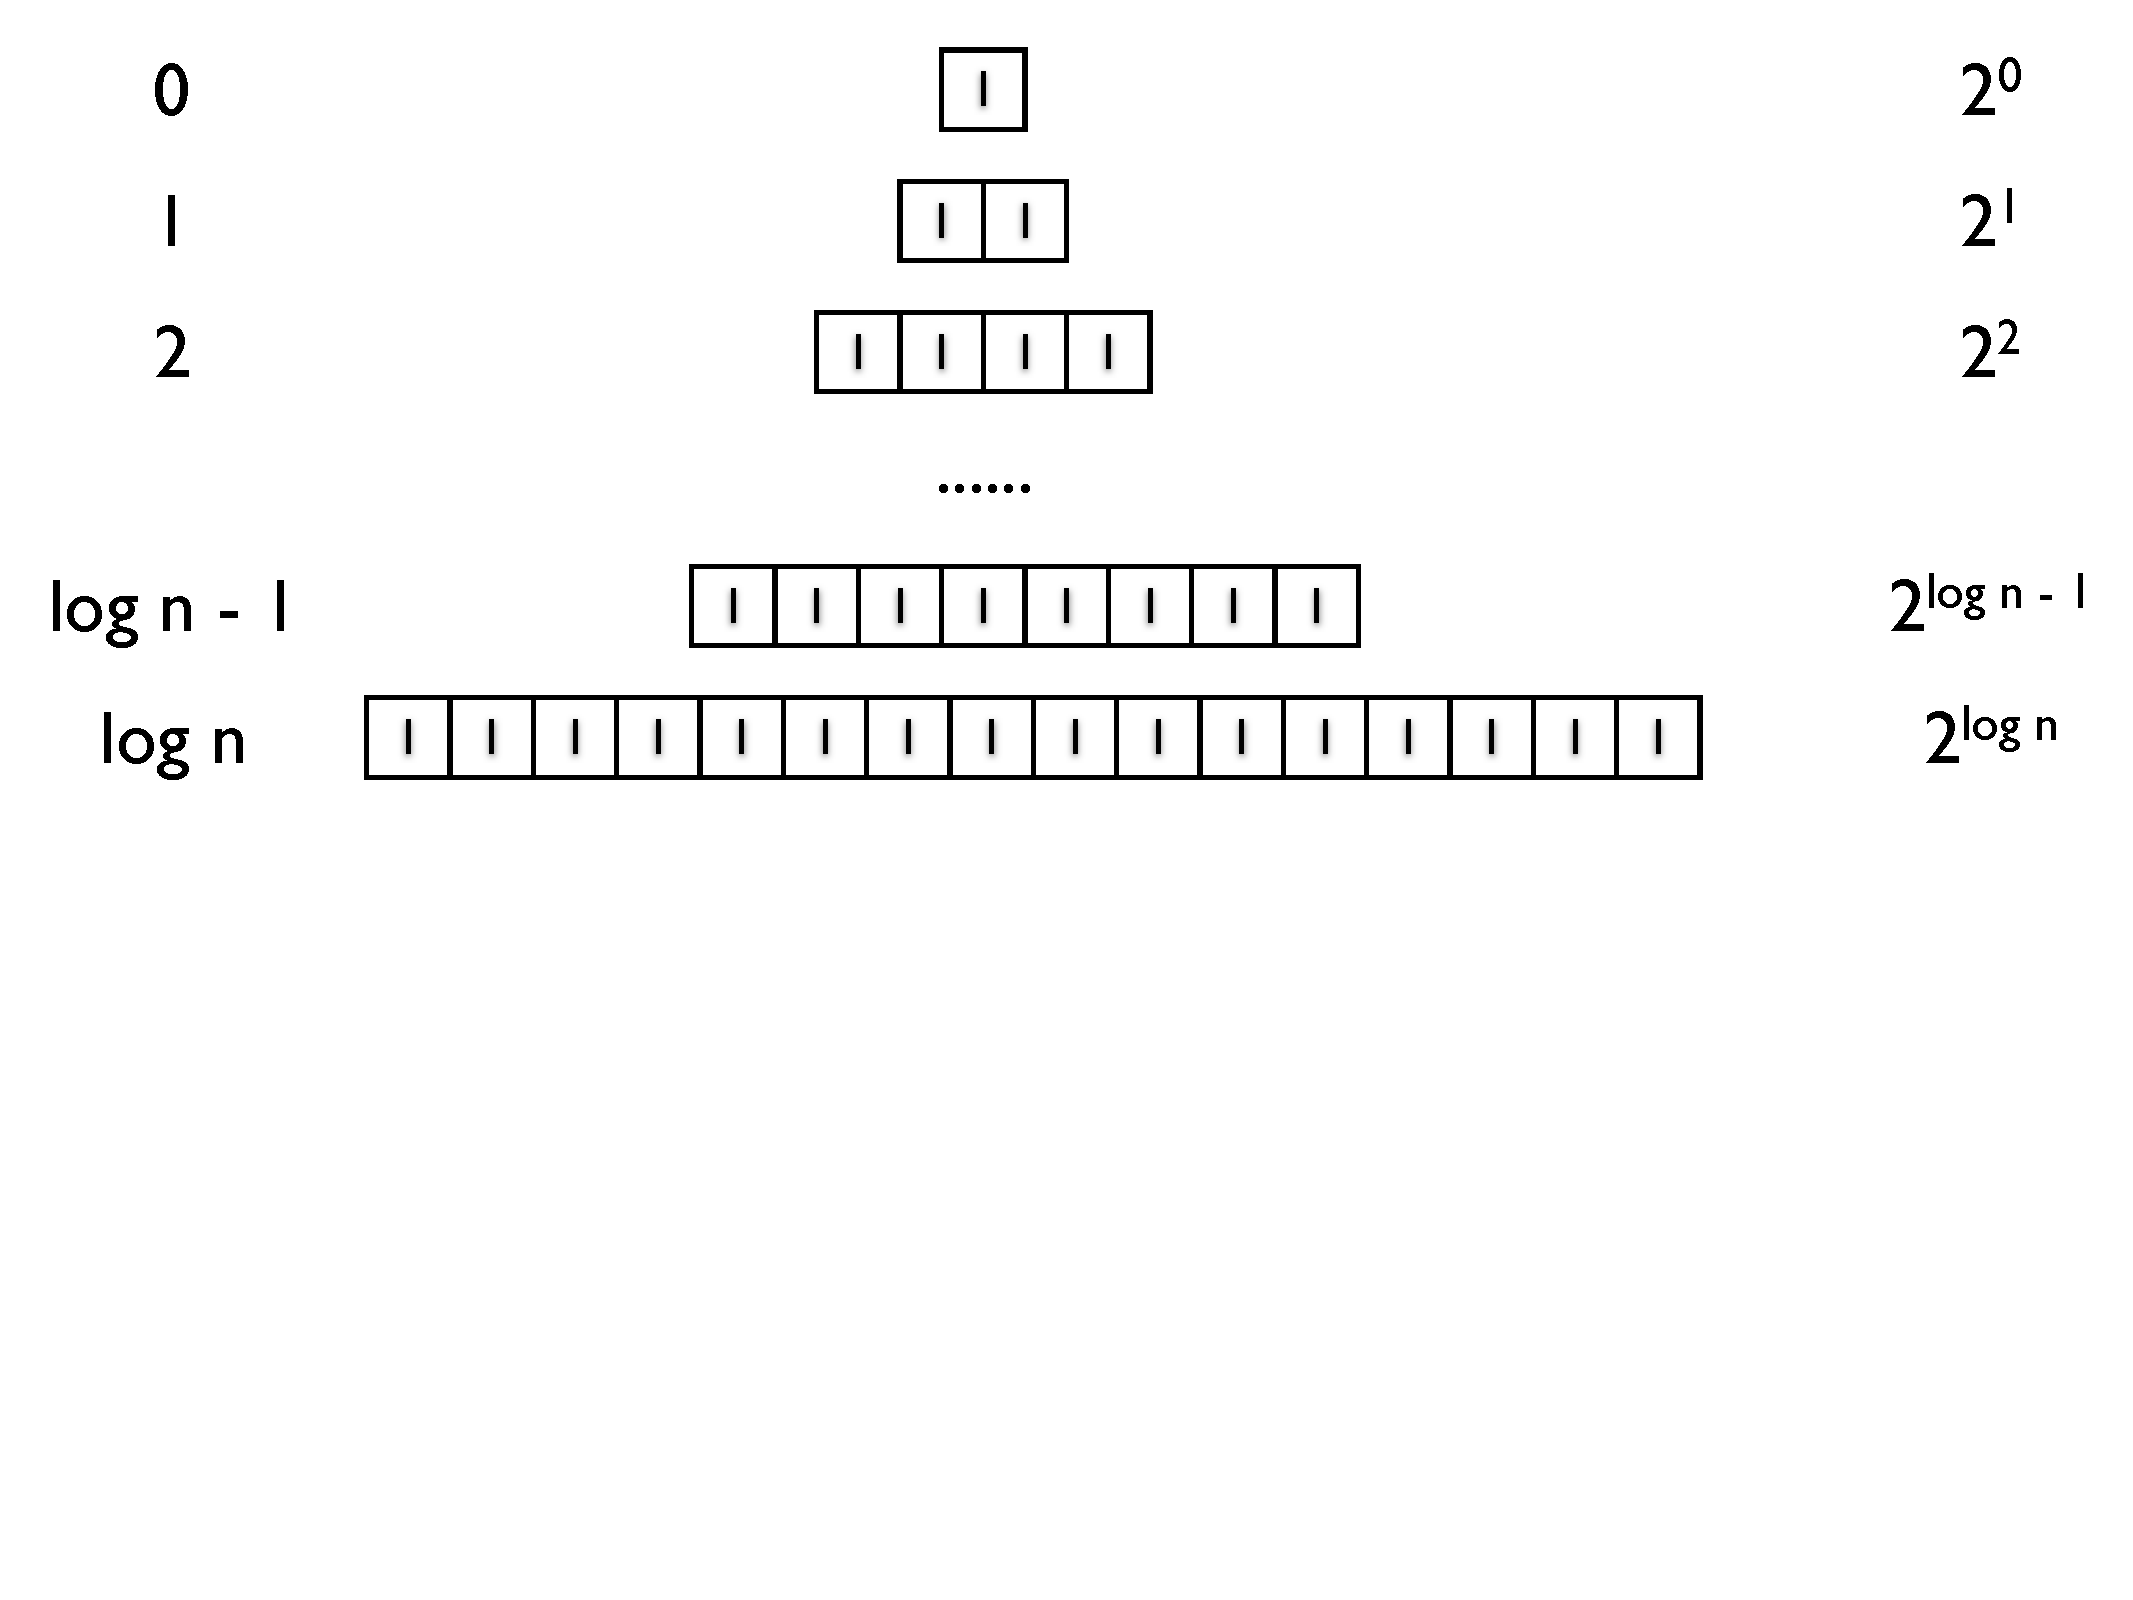
\includegraphics[width=.6\textwidth]{tree1}
	\caption[]{Rappresentazione della ricorsione.}
\end{figure}

\[
	T(n) = \sum_{i=0}^{\log n} 2^i = n + \frac{n}{2} + \frac{n}{4} + \cdots + 1 = \Omicron(n)
\]

Effettuiamo un tentativo per \fbox{\(T(n) = \Omicron(n)\)}

\begin{itemize}
	\item \textbf{ipotesi induttiva}: \(\forall k < n \,\colon T(k) \leqslant ck\).
	\item \textbf{passo induttivo}: dimostriamo la disequazione per \(T(n)\):
	\clearpage
	\[\begin{WithArrows}
	T(n) &= T(\floor{ \frac{n}{2} }) + T(\ceil{ \frac{n}{2} }) + 1 \Arrow{sost. ip. ind.}\\
		 &= c(\floor{ \frac{n}{2} }) + c(\ceil{ \frac{n}{2} }) + 1 \Arrow{semplifichiamo, \(\floor{ \frac{n}{2} } + \ceil{ \frac{n}{2} } = n\)}\\
		 &= cn + 1 \Arrow{obiettivo}\\
		 &= cn + 1 \overset{?}{\leqslant} cn \Arrow{semplifico}\\
		 &\Rightarrow 1 \leqslant 0
	\end{WithArrows}\]

	Anche in questo caso notiamo che l'ultima disequazione risulta impossibile, ma \mbox{--- a differenza del caso precendente ---} non riusciamo a dimostrare il passo induttivo per un termine di ordine inferiore.
	Il tentativo risulta quindi errato.

	Proviamo quindi ad utilizzare un'ipotesi induttiva \emph{più stretta}.

	\item \textbf{ipotesi induttiva più stretta}: \(\exists c > 0, \exists m \geqslant 0 \,\colon T(n) \leqslant cn - b, \forall n \geqslant m\), \(b > 0\).

	Abbiamo introdotto una costante \(b > 0\) nella nostra tesi, questa modifica ci permetterà di dimostrare correttamente il passo induttivo.

	\item \textbf{ipotesi induttiva} \(\exists b > 0, \forall k < n \,\colon T(k) \leqslant ck - b\).

	\item \textbf{passo induttivo} dimostriamo la disequazione per \(T(n)\):
	\[\begin{WithArrows}
	T(n) &= T(\floor{ \frac{n}{2} }) + T(\ceil{ \frac{n}{2} }) + 1 \Arrow{sost. ip. ind.}\\
	&= c(\floor{ \frac{n}{2} }) - b + c(\ceil{ \frac{n}{2} }) - b + 1 \Arrow{semplifichiamo}\\
	&= cn -2b + 1 \Arrow{obiettivo}\\
	&= cn -2b + 1 \overset{?}{\leqslant} cn - b\Arrow[jump=2]{semplifico}\\
	&\Leftrightarrow -2b + 1 \leqslant -b\\
	&\Leftrightarrow b \geqslant 1
	\end{WithArrows}\]

	\item \textbf{caso base}
	\[T(1) = 1 \overset{?}{\leqslant} c \cdot 1 - b \Leftrightarrow c \geqslant b + 1\]
	Per concludere abbiamo provato che \(T(n) \leqslant cn - b \leqslant cn\) con diversi valori delle costanti \(c\) e \(b\), nel passo induttivo \(\forall b \geqslant 1, \forall c\), nel caso base \(\forall c \geqslant b+1\).
	Una coppia di valori di \(b\) e \(c\) che rispettano queste disequazioni sono \(b = 1\), \(c = 2\).

	Questo vale per \(n = 1\), e per tutti i valori di \(n\) successivi, quindi per \(m = 1\).

	Abbiamo quindi provato che \(T(n) = \Omicron(n)\).
\end{itemize}

Dimostriamo il limite inferiore facendo un tentativo per \fbox{\(T(n) = \Omega(n)\)}

Dobbiamo dimostrare che \(\exists d > 0, \exists m \geqslant 0 \,\colon T(n) \geqslant dn, \forall n \geqslant m\).

\begin{itemize}
	\item \textbf{passo induttivo}
	\[\begin{WithArrows}
	T(n) &= T(\floor{ \frac{n}{2} }) + T(\ceil{ \frac{n}{2} }) + 1 \Arrow{sost. ip. ind.}\\
	&\geqslant d(\floor{ \frac{n}{2} }) + d(\ceil{ \frac{n}{2} }) + 1 \Arrow{semplifichiamo}\\
	&= dn + 1 \Arrow{obiettivo}\\
	&= dn + 1 \overset{?}{\geqslant} dn
	\end{WithArrows}\]
	L'ultima disequazione risulta vera \(\forall d\).
	\item \textbf{caso base}
	\[T(n) = 1 \geqslant d \cdot 1 \iff d \leqslant 1\]

	Abbiamo quindi provato che \(T(n) = \Omega(n)\)
\end{itemize}

\subsection*{Problemi con i casi base}

\[
	T(n) =
	\begin{cases}
		2T(\floor{ \frac{n}{2} }) + n & n > 1 \\
		1 & n \leqslant 1
	\end{cases}
\]
Proviamo a visualizzarlo graficamente così:

\begin{figure}[H]
	\centering
	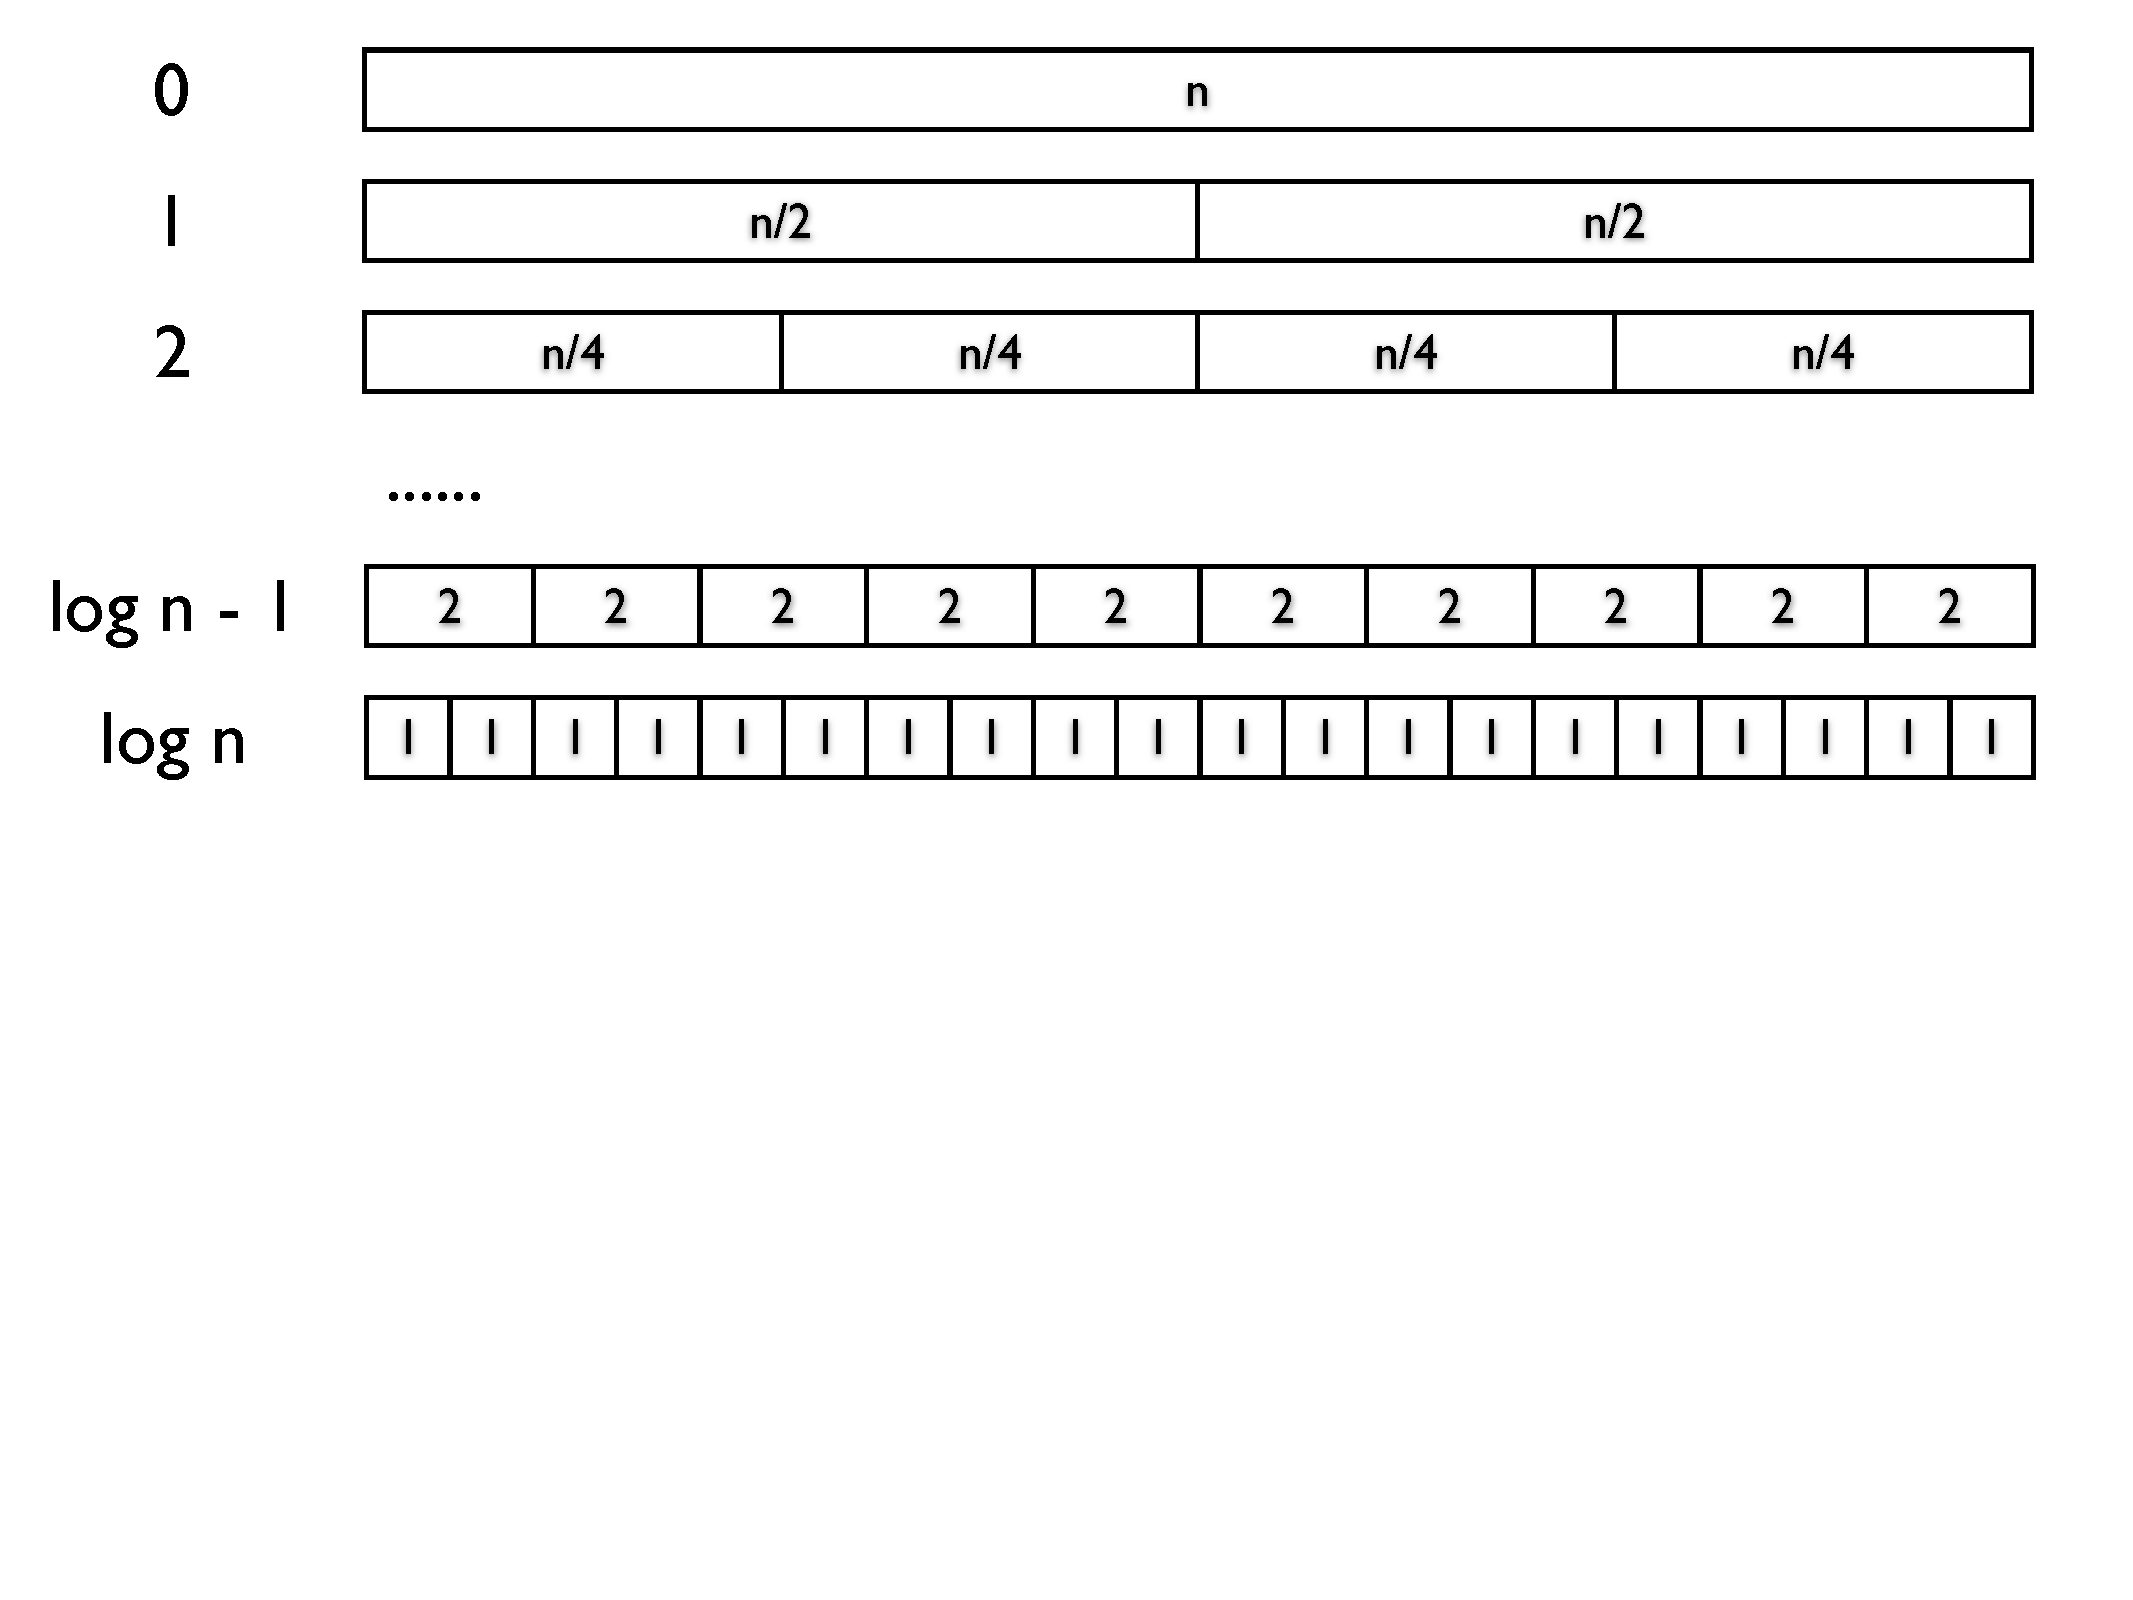
\includegraphics[width=.6\textwidth]{mergesort}
	\caption[]{Rappresentazione della ricorsione.}
\end{figure}

\begin{note}
\`{E} molto simile all'equazione dell'algoritmo \mergeSort che sappiamo avere una complessità di \(\Omicron(n \log n)\).
\end{note}

Effettuiamo un tentativo per \fbox{\(T(n) = \Omicron(n \log n)\)}

Dobbiamo dimostrare che \(\exists c > 0, \exists m \geqslant 0 \,\colon T(n) \leqslant cn \log n, \forall n \geqslant m\).

\begin{itemize}
	\item \textbf{Ipotesi induttiva}: \(\exists c > 0, \forall k < n \,\colon T(k) \leqslant ck \log k\)
	\item \textbf{Passo di induzione}: Dimostriamo la disequazione per \(T(n)\):
	\[\begin{WithArrows}
	T(n) &= 2T(\floor{ \frac{n}{2} }) + n \Arrow{sost. ip. ind. con \(k = \floor{\frac{n}{2}}\)}\\
		 &\leqslant 2c\floor{ \frac{n}{2} } \log \floor{ \frac{n}{2} } + n \Arrow{rimuovo l'intero inferiore}\\
		 &\leqslant \Ccancel{2}c \frac{n}{\Ccancel{2}} \log \frac{n}{2} + n \Arrow{semplifico}\\
		 &= cn \log \frac{n}{2} + n \Arrow{\(\log \frac{n}{2} = \log n - \log_2 2 = \log n - 1\)}\\
		 &= cn (\log n - 1) + n \Arrow{moltiplico}\\
		 &= cn \log n - cn + n \Arrow{obiettivo}\\
		 &\leqslant cn \log n - cn + n \overset{?}{\leqslant} cn \log n \Arrow[jump=2]{semplifico}\\
		 &\Leftrightarrow -cn + n \leqslant 0\\
		 &\Leftrightarrow c \geqslant 1
	\end{WithArrows}\]
	\item \textbf{caso base}: dimostriamo la disequazione per \(T(1)\)
	\[T(1) = 1 \overset{?}{\leqslant} 1 \cdot c \log 1 = 0 \Rightarrow 1 \nleq 0\]
	\`{E} falso, ma non è un problema, non a caso si chiama notazione asintotica: il valore di \(m\) lo possiamo scegliere noi.
	\item \textbf{caso base}: dimostriamo la disequazione per \(T(2)\), \(T(3)\)
	\begin{align*}
		T(2) &= 2T(\floor{\frac{2}{2}}) + 2 = 4 \leqslant 1 \cdot c \cdot 2 \log 2 \Leftrightarrow c \geqslant 2\\
		T(3) &= 2T(\floor{\frac{3}{2}}) + 3 = 5 \leqslant 1 \cdot c \cdot 3 \log 3 \Leftrightarrow c \geqslant \frac{5}{3 \log 3}\\
		T(4) &= 2T(\floor{\frac{4}{2}}) + 4 = 2T(\floor{2}) + 4
	\end{align*}
	Non è necessario provare la terza disequazione, in quanto viene espressa in base ai casi base diversi da \(T(1)\) che sono già stati dimostrati e quindi possono costituire la base per la nostra induzione.
\end{itemize}

Riassumendo:
\begin{itemize}
	\item[] Abbiamo provato che \(T(n) \leqslant cn \log n\)
	\begin{itemize}[label=\textbullet]
		\item nel passo induttivo: \(\forall c \geqslant 1\)
		\item nel caso base: \(\forall c \geqslant 2, c \geqslant \frac{5}{3\log 3}\)
	\end{itemize}
	Visto che sono tutte disequazioni con il segno \(\geqslant\), è sufficiente utilizzare \(c \geqslant \maxFunction\left\{ 1,2,\frac{5}{3 \log 3} \right\}\)

	Questo vale per \(n=2\), \(n=3\), e per tutti i valori di \(n\) successivi, quindi \(m = 2\).
\end{itemize}

\subsection*{Ultimo esercizio}

\[
	T(n) =
	\begin{dcases}
	9 T( \floor{\nicefrac{n}{3} }) + n & n > 1 \\
	1 & n \leqslant 1 \\
	\end{dcases}
\]

Effettuiamo un tentantivo \fbox{\(T(n) = \Omicron(n^2)\)}

Dobbiamo dimostrare che \(\exists c > 0, \exists m \geqslant 0 \,\colon T(n) \leqslant cn^2, \forall n \geqslant m\)
\begin{itemize}
	\item \textbf{ipotesi induttiva}: \(\exists c > 0 \,\colon T(k) \leqslant ck^2, \forall k < n\)
	\item \textbf{passo induttivo} dimostriamo la disequazione per \(T(n)\):
	\[\begin{WithArrows}
	T(n) &= 9T\left( \floor{\frac{n}{3}} \right) + n \Arrow{sost. ip. ind. con \(k = \floor{\frac{n}{3}}\)}\\
		 &\leqslant 9 c{\left( \floor{\frac{n}{3}} \right)}^{2} + n \Arrow{rimuovo l'intero inferiore}\\
		 &\leqslant 9 c \left( \frac{n^2}{9} \right) + n \Arrow{semplifico il \(9\)}\\
		 &= cn^2 + n \Arrow{obiettivo}\\
		 &= cn^2 + n \leqslant cn^2
	\end{WithArrows}\]
	L'ultima disequazione risulta falsa per un termine di ordine inferiore: proviamo quindi a modificare l'ipotesi induttiva e a ripetere il passo induttivo.
	\item \textbf{ipotesi induttiva più stretta} \(\exists c > 0 \,\colon T(k) \leqslant c(k^2 - k), \forall k < n\)
	\item \textbf{passo induttivo} dimostriamo la disequazione per \(T(n)\):
	\[\begin{WithArrows}
	T(n) &= 9T\left( \floor{\frac{n}{3}} \right) + n \Arrow{sost. ip. ind. con \(k = \floor{\frac{n}{3}}\)}\\
		 &\leqslant 9c \left( {\floor{\frac{n}{3}}}^{2} - \floor{\frac{n}{3}} \right) + n \Arrow{rimuovo l'intero inferiore}\\
		 &\leqslant 9c \left( {\left(\frac{n}{3}\right)}^{2} - \frac{n}{3} \right) + n \Arrow{svolgo la potenza}\\
		 &\leqslant 9c \left( \frac{n^2}{9} - \frac{n}{3} \right) + n \Arrow{moltiplico}\\
		 &\leqslant cn^2 - 3cn + n \Arrow{obiettivo}\\
		 &\leqslant cn^2 - 3cn + n \overset{?}{\leqslant} cn^2 - cn \Arrow[jump=2]{semplifico}\\
		 &\Leftrightarrow 2 cn \geqslant cn\\
		 &\Leftrightarrow c \geqslant \frac{1}{2}
	\end{WithArrows}\]
	\item \textbf{caso base}
	\begin{align*}
		T(1) &= 1 \leqslant c(1^2 - 1) = 0, falso\\
		T(2) &= 9T(0) + 2 = 11 \leqslant c(2^2 - 2) \Leftrightarrow c \geqslant \nicefrac{11}{2}\\
		T(3) &= 9T(1) + 3 = 12 \leqslant c(3^2 - 3) \Leftrightarrow c \geqslant \nicefrac{12}{6}\\
		T(4) &= 9T(1) + 4 = 13 \leqslant c(4^2 - 4) \Leftrightarrow c \geqslant \nicefrac{13}{12}\\
		T(5) &= 9T(1) + 5 = 14 \leqslant c(5^2 - 5) \Leftrightarrow c \geqslant \nicefrac{14}{20}\\
		T(6) &= 9T(2) + 6
	\end{align*}
	Non è necessario andare oltre poiché T(6) dipende da T(2) che è già stato dimostrato.

	Riassumendo i parametri scelti sono:
	\begin{itemize}[label=\textbullet]
		\item \(c \geqslant \maxFunction \left\{ \frac{1}{2},\frac{11}{2},\frac{12}{6},\frac{13}{12},\frac{14}{20} \right\}\)
		\item \(m = 1\)
	\end{itemize}
	Nota che l'esempio combina le due difficoltà insieme, ma è stato creato artificiosamente: infatti se avessimo scelto come ipotesi più stretta \(T(n) \leqslant cn^2 - bn\), il problema sui casi base non si sarebbe posto.

	Abbiamo quindi dimostrato che \(T(n) \leqslant c(n^2 - n) \leqslant cn^2, \forall n \geqslant 1, \forall c \geqslant \frac{14}{20}\), ossia che \(T(n) = \Omicron(n)\)
\end{itemize}

\subsection*{Riassumendo}

Il metodo di sostituzione è composto da tre parti:
\begin{enumerate}
	\item si \emph{indovina} una possibile soluzione e si formula un'ipotesi induttiva;
	\item si \emph{sostituisce} nella ricorrenza le espressioni \(T(\,\cdot\,)\), utilizzando l'ipotesi induttiva;
	\item si \emph{dimostra} che la soluzione è valida anche per il caso base.
\end{enumerate}

Bisogna fare attenzione:
\begin{itemize}
	\item ad ipotizzare soluzioni troppo \enquote{strette};
	\item ad alcuni casi particolari che richiedono astuzie matematiche;
	\item ai casi base in cui compare il logaritmo in quanto potrebbe complicare le cose.
\end{itemize}

\clearpage
\section{Metodo dell'esperto (o delle ricorrenze comuni)}

Esiste un'ampia classe di ricorrenze che possono essere risolte facilmente facendo ricorso ad alcuni teoremi, ognuno dei quali si occupa di una classe particolare di equazioni di ricorrenza.

\begin{theorem}[ricorrenze lineari con partizione bilanciata]
Siano \(a\) e \(b\) costanti intere tale che \(a \geqslant 1\) e \(b \geqslant 2\), e \(c\), \(\beta\) costanti reali tali che \(c > 0\) e \(\beta \geqslant 0\).
Sia \(T(n)\) data dalla relazione di ricorrenza:
\[
	T(n) =
	\begin{dcases}\textstyle
		a\T{\frac{n}{b}} + cn^{\beta} & n > 1 \\
		d & n \leqslant 1 \\
	\end{dcases}
\]
Posto \(\alpha = \frac{\log a}{\log b} = \log_{b} a\), allora:
\[
	T(n) =
	\begin{dcases}
		\Theta(n^{\alpha}) & \alpha > \beta \\
		\Theta(n^{\alpha}\log n) & \alpha = \beta \\
		\Theta(n^{\beta}) & \alpha < \beta \\
	\end{dcases}
\]
\end{theorem}

\paragraph{Commento}
Affrontiamo le equazioni di ricorrenza in cui la dimensione viene divisa in \(b\) parti, dove \(b\) dev'essere almeno pari a 2; l'algoritmo ricorsivo dev'essere richiamato \(a\) volte, dove \(a\) è almeno 1.
Nella versione estesa, che vedremo fra poco, vedremo che i parametri \(a\) e \(b\) verranno \enquote{rilassati}.

Prendiamo ad esempio il primo esercizio \(T(n) = 4T(\frac{n}{2})\) e vediamo che si può risolvere semplicemente calcolando \(\alpha = \log_b a = \log_2 4 = 2 > \beta = 1\), possiamo quindi concludere che \(T(n) = \Theta(n^{\alpha}) = \Theta(n^2)\).

\begin{proof}[teorema delle ricorrenze lineari con partizione bilanciata]
Assumiamo che \(n\) sia una potenza intera di \(b\), ossia che \(n = b^k\), \(k = \log_b n\) poiché ci permetterà di semplificare i calcoli successivi ed è ininfluente sul risultato.
Ad esempio supponiamo che l'input abbia dimensione \(b^k + 1\) (\(2^8 + 1 = 257\) bit), se estendiamo l'input fino ad una dimensione \(b^{k+1}\) (\(2^8+1 = 512\) bit, facendo del \foreign{padding}, l'input sarebbe stato esteso al massimo di un fattore costante \(b\) (\(2\) nel nostro caso), il che è ininfluente al fine della complessità computazionale.

Calcoliamo l'albero delle ricorrenze per la seguente equazione di ricorrenza:
\[
	T(n) =
	\begin{dcases}\textstyle
		a\T{\frac{n}{b}} + cn^{\beta} & n > 1 \\
		d & n \leqslant 1 \\
	\end{dcases}
\]

\clearpage
\begin{center}
	\begin{tabular}{@{} *{5}{c} @{}}
		\toprule
			livello & dim. & costo chiam. & no. chiamate & costo livello \\
		\midrule
			\(0\) & \(b^k\) & \(c\,b^{k\beta}\) & \(1\) & \(cb^{k\beta}\) \\
		\addlinespace
			\(1\) & \(b^{k-1}\) & \(c\,b^{(k-1)\beta}\) & \(a\)  & \(a \cdot c\, b^{(k-1)\beta}\)\\
		\addlinespace
			\(2\) & \(b^{k-2}\) & \(c\,b^{(k-2)\beta}\) & \(a^2\) & \(a^2 \cdot c\, b^{(k-2)\beta}\)\\
		\addlinespace
			\(\vdots\) & \(\vdots\) & \(\vdots\) & \(\vdots\) & \(\vdots\) \\
		\addlinespace
			\(i\) & \(b^{k-i}\) & \(c\,b^{(k-i)\beta}\) & \(a^i\) & \(a^i \cdot c\, b^{(k-i)\beta}\)\\
		\addlinespace
			\(\vdots\) & \(\vdots\) & \(\vdots\) & \(\vdots\) & \(\vdots\) \\
		\addlinespace
			\(k-1\) & \(b\) & \(c b^{(k-(k-1))\beta} = c\,b^{\beta}\) & \(a^{k-1}\) & \(a^{k-1} \cdot c\, b^{\beta}\) \\
		\addlinespace
			\(k\) & \(1\) & \(d\) & \(a^k\) & \(a^k \cdot d\) \\
		\bottomrule
	\end{tabular}
\end{center}

Sommando i costi totali del \(k\)-esimo livello e dei livelli fino al \(k-1\), si ottiene:
\[\begin{WithArrows}[displaystyle]
T(n) &= da^k + \sum_{i=0}^{k-1} a^i \cdot c b^{(k-i)\beta} \Arrow{moltiplico}\\
	 &= da^k + \sum_{i=0}^{k-1} a^i \cdot c b^{k\beta} \cdot b^{-i\beta} \Arrow{porto fuori i termini\\non dipendenti da \(i\)}\\
	 &= da^k + cb^{k\beta} \sum_{i=0}^{k-1} \frac{a^i}{b^{i\beta}} \Arrow{raccolgo \(i\)}\\
	 &= da^k + cb^{k\beta} \sum_{i=0}^{k-1} \left( \frac{a}{b^{\beta}} \right)^{i}
\end{WithArrows}\]
A questo punto ho una formula chiusa ma non ancora nella sua forma definitiva.

\
Facciamo alcune osservazioni.
\begin{itemize}[label=\textbullet]
	\item \(a^k = a^{\log_b n} = a^{\frac{\log n}{\log b}} = 2^{\log_2 a \frac{\log n}{\log b}} = 2^{\log_2 n \frac{\log a}{\log b}} = n^{\frac{\log a}{\log b}} = n^{\alpha}\)

	\item \(\alpha = \frac{\log a}{\log b} \Leftrightarrow \alpha\log b = \log a \Leftrightarrow \log b^{\alpha} = \log a \Leftrightarrow a = b^{\alpha}\)

	\item poniamo \(q = \frac{a}{b^{\beta}} = \frac{b^{\alpha}}{b^{\beta}} = b^{\alpha-\beta}\)
\end{itemize}
Grazie alle osservazioni appena fatto possiamo sostituire i parametri nell'equazione finale:
\[\begin{WithArrows}[displaystyle]
T(n) &= da^k + cb^{k\beta} \sum_{i=0}^{k-1} \left( \frac{a}{b^{\beta}} \right)^{i} \Arrow{sostituisco: \(\alpha^k \rightarrow n^{\alpha}\)\\sostituisco: \(a \rightarrow b^{\alpha}\), \(q = \frac{b^{\alpha}}{b^{\beta}}\)}\\
	 &= dn^{\alpha} + cb^{k\beta} \sum_{i=0}^{k-1} q^{i}
\end{WithArrows}\]
Da qui si aprono tre possibilità, ossia che
\begin{enumerate*}
	\item \(\alpha > \beta\)
	\item \(\alpha = \beta\)
	\item \(\alpha < \beta\)
\end{enumerate*}
Studiamole una per una.

\begin{enumerate}
	\item Caso \fbox{\(\alpha > \beta\)}, ne segue che \(q = b^{\alpha - \beta} > 1\)
	\[\begin{WithArrows}[displaystyle]
	T(n) &= dn^{\alpha} + cb^{k\beta} \sum_{i=0}^{k-1} q^{i} \Arrow{serie geometrica finita}\\
		 &= n^{\alpha}d + cb^{k\beta} \left[ \frac{q^k - 1}{q-1} \right] \Arrow{introduco la disequazione}\\
		 &\leqslant n^{\alpha}d + cb^{k\beta} \frac{q^k}{q-1} \Arrow{sostituisco: \(q = \frac{a}{b^{\beta}} \Rightarrow q^k = \frac{a^k}{b^{k\beta}}\)}\\
		 &= n^{\alpha}d + \frac{cb^{k\beta}a^k}{b^{k\beta}} \frac{1}{q-1} \Arrow{semplifico: \(b^{k\beta}\)}\\
		 &= n^{\alpha}d + \frac{ca^k}{q-1} \Arrow{sostituisco: \(a^k = n^{\alpha}\)}\\
		 &= n^{\alpha}d + \frac{cn^{\alpha}}{q-1} \Arrow{raccolgo per \(n^{\alpha}\)}\\
		 &= n^{\alpha} \left[ d + \frac{c}{q-1} \right]
	\end{WithArrows}\]
	Visto che \(d\), \(c\) e \(q\) sono tutti termini positivi e costanti possiamo concludere che \(n^{\alpha}\) limita superiormente l'espressione e che quindi \(T(n) = \Omicron(n^{\alpha})\).
	Infine per via della componente non ricorsiva \(dn^{\alpha}\), \(T(n)\) è anche \(\Omega(n^{\alpha})\), possiamo concludere che \(T(n) = \Theta(n^{\alpha})\).

	\item Caso \fbox{\(\alpha = \beta\)}, ne segue che \(q = b^{\alpha - \beta} = 1\)
	\[\begin{WithArrows}[displaystyle]
	T(n) &= dn^{\alpha} + cb^{k\beta} \sum_{i=0}^{k-1} q^{i} \Arrow{\(q^i = 1^i = 1\)\\\(1+2+\cdots+k-1 = k\)}\\
		 &= n^{\alpha}d + cn^{\beta}k \Arrow{sostituisco: \(\beta = \alpha\)}\\
		 &= n^{\alpha}d + cn^{\alpha}k \Arrow{raccolgo per \(n^{\alpha}\)}\\
		 &= n^{\alpha}(d + ck) \Arrow{sostituisco: \(k = \log_b n\)}\\
		 &= n^{\alpha}(d + c\textstyle\frac{\log n}{\log b})
	\end{WithArrows}\]
	Visto che \(d\), \(c\) e \(\log b\) sono tutti termini positivi e costanti e che non abbiamo introdotto disequazioni, possiamo affermare che \(T(n) = \Theta(n^{\alpha}\log n)\).

	\item Caso \fbox{\(\alpha < \beta\)}, ne segue che \(q = b^{\alpha - \beta} < 1\)
	\[\begin{WithArrows}[displaystyle]
	T(n) &= dn^{\alpha} + cb^k \sum_{i=0}^{k-1} q^i \Arrow{serie geometrica finita}\\
		 &= dn^{\alpha} + cb^k \left[ \frac{q^k - 1}{q-1} \right] \Arrow{inversione, \(1-q > 0\)}\\
		 &= dn^{\alpha} + cb^k \left[ \frac{1 - q^k}{1-q} \right] \Arrow{introduco\\la disequazione}\\
		 &\leqslant dn^{\alpha} + cb^k \left[ \frac{1}{1-q} \right] \Arrow{sostituisco: \(b^k = n\)}\\
		 &= n^{\alpha}d + \frac{cn^{\beta}}{1-q}
	\end{WithArrows}\]
	\(n^{\alpha} < n^{\beta}\) quindi considero il polinomio di grado maggiore, di conseguenza \(T(n)\) è \(\Omicron(n^{\beta})\).
	Poiché \(T(n) = \Omega(n^{\beta})\) per via del termine non ricorsivo, possiamo affermare che \(T(n) = \Theta(n^{\beta})\).
\end{enumerate}
Fine dimostrazione.
\end{proof}

\begin{theorem}[ricorrenze lineari con partizione bilanciata estesa]
Sia \(a \geqslant 1\), \(b > 1\), \(f(n)\) asintoticamente positiva, e sia
\[
	T(n) =
	\begin{dcases}\textstyle
		a\T{\frac{n}{b}} + f(n) & n > 1 \\
		d & n \leqslant 1 \\
	\end{dcases}
\]
Sono dati tre casi:
\begin{enumerate}
	\item \(\exists \varepsilon > 0 \colon f(n) = \Omicron(n^{\alpha-\varepsilon})\) allora \(T(n) = \Theta(n^{\alpha})\);
	\item \(f(n) = \Theta(n^\alpha)\) allora \(T(n) = \Theta(f(n)\log n)\);
	\item \(\exists \varepsilon > 0 \,\colon f(n) = \Omicron(n^{\alpha + \varepsilon}) \land\\\exists c \,\colon 0 < c < 1, \exists m > 0 \,\colon\\a f(\frac{n}{b}) \leqslant c f(n), \forall n \geqslant m\) allora \(T(n) = \Theta(f(n))\).
\end{enumerate}
\end{theorem}

Non vedremo la dimostrazione poiché è troppo complessa.

\paragraph{Commento}
Il teorema precendente funzionava con \(n^{\beta}\), aveva una serie di condizioni semplificative, ora non ci sono più.
Nel secondo caso se \(f(n) = n^{\beta}\) ritorniamo esattamente al secondo caso del teorema precendente, ma qui possiamo prendere in considerazione funzioni più complesse.

\subsection*{Esercizi}

Le soluzioni sono indicate fra parentesi.
\begin{itemize}
	\item \(T(n) = 9T(\frac{n}{3}) + n\) \hfill[\(\Omicron(n^{2-\varepsilon})\), con \(\varepsilon < 1\)]
	\item \(T(n) = T(\frac{2}{3} n) + 1\)  \hfill[\(\Theta(n^0)\)]
	\item \(T(n) = 3T(\frac{n}{4}) + n\log n\) \hfill[\(c = \nicefrac{3}{4}\), \(m = 1\)]
	\item \(T(n) = 2T(\frac{n}{2}) + n\log n\) \hfill[nessun caso applicabile]
\end{itemize}

\begin{theorem}[ricorrenze lineari di ordine costante]
Siano \(\{a_1, a_2, \dots, a_n\}\) costanti intere non negative, con \(h\) costante positiva, \(c\) e \(\beta\) costanti reali tali che \(c > 0\) e \(\beta \geqslant 0\), e sia \(T(n)\) definita dalla relazione di ricorrenza:
\[
	T(n) =
	\begin{dcases}
		\sum_{1 \leqslant i \leqslant h} a_i \T{n-1} + cn^{\beta} & n > m \\
		\Theta(1) & n \leqslant m \leqslant h \\
	\end{dcases}
\]
Posto \(a = \sum_{1 \leqslant i \leqslant h} a_i\), allora:
\begin{enumerate}
	\item \(T(n)\) è \(\Theta(n^{\beta+1})\), se \(a = 1\);
	\item \(T(n)\) è \(\Theta(a^n n^{\beta})\), se \(a \geqslant 2\).
\end{enumerate}
\end{theorem}

\paragraph{Commento}
Questo teorema tratta ricorrenze lineari \emph{di ordine costante} perché tutte le volte rimuoviamo dalla dimensione di input \(n\) una quantità costante.

\subsection*{Esercizi}

Le soluzioni sono indicate fra parentesi.
\begin{itemize}[label=\textbullet]
	\item \(T(n) = T(n-10) + n^2\) \hfill[costo polinomiale]
	\item \(T(n) = T(n-2) - T(n-1) + 1\) \hfill[costo esponenziale]
\end{itemize}

\section{Algoritmo della somma massimale di un sottovettore}

Date le nostre nuove conoscenze possiamo calcolare con precisione la complessità delle varie versioni degli algoritmi proposti per la soluzione al problema della somma massimale di un sottovettore.

\subsubsection*{Complessità della prima versione}

\begin{code}
\begin{minted}{cpp}
int maxsum1(int[] A, int n) {
	int maxSoFar = 0;
	for (int i = 0; i < n; i++) {
		for (int j = i; j < n; j++) {
			int sum = 0;
			for (int k = i; k <= j; k++) {
				sum = sum + A[k];
			}
			maxSoFar = max(maxSoFar, sum);
		}
	}
	return maxSoFar;
}
\end{minted}
% \captionof{listing}{Versione 1}
% \label{code:c-code}
\end{code}

La complessità dell'algoritmo può essere approssimata come segue (contando il numero di esecuzioni della riga più interna):
\[\begin{WithArrows}[displaystyle]
T(n) = \sum_{i=0}^{n-1} \sum_{j=i}^{n-1} (j - i + 1)
\end{WithArrows}\]

Vogliamo provare che \(T(n) = \Omicron(n^3)\).
\begin{proof}
\textbf{limite superiore}:
\(\exists c_2 > 0, \exists m \geqslant 0 : T(n) \leqslant c_2 n^3\), \(\forall n \geqslant m\).
\[\begin{WithArrows}[displaystyle]
T(n) &= \sum_{i=0}^{n-1} \sum_{j=i}^{n-1} (j - i + 1) \Arrow{spiegazione}\\
	 &\leqslant \sum_{i=0}^{n-1} \sum_{j=i}^{n-1} n \Arrow{spiegazione}\\
	 &\leqslant \sum_{i=0}^{n-1} \sum_{j=0}^{n-1} n \Arrow{spiegazione}\\
	 &=\sum_{i=0}^{n-1} n^2 \Arrow{spiegazione}\\
	 &= n^3 \leqslant c_2 n^3
\end{WithArrows}\]
Questa disequazione è vera per \(n \geqslant m = 0\) and \(c_2 \geqslant 1\).
\end{proof}

Vogliamo provare che \(T(n) = \Omega(n^3)\).
\begin{proof}
\textbf{limite inferiore}:
\(\exists c_1 > 0, \exists m \geqslant 0 : T(n) \leqslant c_1 n^3\), \(\forall n \geqslant m\).
\[\begin{WithArrows}[displaystyle]
T(n) &= \sum_{i=0}^{n-1} \sum_{j=i}^{n-1} (j - i + 1) \\
	 &\geqslant \sum_{i=0}^{\nicefrac{n}{2}} \sum_{j=i}^{n+\nicefrac{n}{2}-1} (j - i + 1) \Arrow{spiegazione}\\
	 &= \sum_{i=0}^{\nicefrac{n}{2}} \sum_{j=i}^{n+\nicefrac{n}{2}-1} \nicefrac{n}{2} \Arrow{spiegazione}\\
	 &= \sum_{i=0}^{\nicefrac{n}{2}} \nicefrac{n^2}{4} \geqslant \nicefrac{n^3}{8} \geqslant c_1 n^3
\end{WithArrows}\]
Questa disequazione è vera per \(n \geqslant m = 0\) and \(c_1 \geqslant 8\).
\end{proof}

\subsubsection*{Complessità della seconda versione}

\begin{code}
\begin{minted}{cpp}
int maxsum2(int[] A, int n) {
	int maxSoFar = 0;
	for (int i=0; i < n; i++) {
		int sum = 0;
		for (int j=i; j < n; j++) {
			sum = sum + A[j];
			maxSoFar = max(maxSoFar, sum);
		}
	}
	return maxSoFar;
}
\end{minted}
% \captionof{listing}{Versione 2}
% \label{code:version-2}
\end{code}

La complessità di questo algoritmo può essere approssimata come segue (stiamo contando il numero di passi nel ciclo più interno):
\[\begin{WithArrows}[displaystyle]
T(n) = \sum_{i=0}^{n-1} n-i
\end{WithArrows}\]

Vogliamo provare che \(T(n) = \Theta(n^2)\)

\begin{proof}
\[\begin{WithArrows}[displaystyle]
T(n) &= \sum_{i=0}^{n-1} n-i \Arrow{spiegazione}\\
     &= \sum_{i=1}^{n} i \Arrow{spiegazione}\\
     &= \frac{n (n + 1)}{2} = \Theta(n^2)
\end{WithArrows}\]
Questo non richiede ulteriori spiegazioni.
\end{proof}

\subsubsection*{Complessità della terza versione}

\begin{code}
\begin{minted}{cpp}
int maxsum_rec(int[] A, int i, int j) {
    if (i == j)
      return max(0, A[i]);

    int m = (i + j) / 2;
    int maxs = maxsum_rec(A, i, m);
    int maxd = maxsum_rec(A, m + 1, j);
    int maxss = 0;
    int sum = 0;

    for (int k = m; k >= i; k--) {
      sum = sum + A[k];
      maxss = max(maxss, sum);
    }

	int maxdd = 0;
    sum = 0;
    for (int k = m + 1; k <= j; k++) {
      sum = sum + A[k];
      maxdd = max(maxdd, sum);
    }

    return max(max(maxs, maxd), maxss + maxdd);
}
\end{minted}
% \captionof{listing}{Versione 3}
% \label{code:version-3}
\end{code}

Per questo, definiamo la equazione di ricorrenza:
\[\begin{WithArrows}[displaystyle]
T(n) = 2T(\nicefrac{n}{2}) + n
\end{WithArrows}\]
Utilizzando il teorema, possiamo vedere che \(\alpha = \log_2 2 = 1\) e \(\beta = 1\), quindi \(T(n) = \Theta(n \log n)\).

\subsubsection*{Complessità della quarta versione}

\begin{code}
\begin{minted}{cpp}
int maxsum4(int A[], int n) {
	int maxSoFar = 0;
	int maxHere = 0;
	for (int i = 0; i < n; i++) {
		maxHere = max(maxHere + A[i], 0);
		maxSoFar = max(maxSoFar, maxHere);
	}

	return maxSoFar;
}
\end{minted}
% \captionof{listing}{Versione 4}
% \label{code:version-4}
\end{code}

\`{E} facile vedere che la complessità di questa versione è \(\Theta(n)\).

\ifsubfile
\end{document}
\fi
